% ------------------------------------------------------------------------
% A Latex template created by Dr. Wenjia Wang for CMP MSc Dissertation. 
% 
% Lasted update: 24/03/2020 by Wenjia Wang
%----------------------------------------------
% Please read the in-file brief Instructions below 
% or More detailed Instructions in sample file (Instrucrtions.tex)
% to learn how to use this option in this template.
% 
% Then go through from current line number 155 to line 205
% to fill in the details about yourself, course, your dissertation, etc. 
%
% Notes and sample files:
% "acronymNotes.tex": brief introduction on how to make a LOA. 
% "acronyms.tex": a sample file where you define abbreviations.
% ------------
% 
% ####---- Brief in-file Instructions ----####
% ----Preparation steps: 
% (i)  Download the zipped Latex templat file into your disk or your university's home space on U disk,
% (ii) Unzip all the fiels into your working folder, such as \Dissertation. 
% (ii) Change/replace/fill some places in this "DissertationTemplate.tex" file to suit your need:
% 	such as, Your course, year, dissertation title, your name, markers, etc.
%
%% Then you can follow teh following instructions(not necessarily in that order) to write your dissertation. 
%   
%% 1. Write your abstract in a provided sample tex file: "Abstract.tex"
%% 2. Write your acknowledgement in a provided sample tex file: "Acknowledgement.tex"  
%    Note: Both tex files are already included in the style file. 
%
%% 3. Write each chapter in a separate tex file and name them e.g. Ch1.tex, Ch2.tex, etc. 
% and then use "include" to inlcude them as shown in this example.
% 
%% 4. Citation styles: package "natbib" is used for making references.
%   you should replace the bib file - xbib, with your own bib file
%   at the END of this template file, i.e.   
%   \bibliography{xbib} % use your own bib file 
%   Then, you can use the following two cammands 
%   to cite your reference, pending on how it is use. 
%   (i) Use Command "\citep{...}" to produce the styyle: (Authors, year)
%   (ii) Use Command "\citet{...}" to produce the style: Authers (year)
%
%#### 
% If you wish to produce a list of abbreviations/acronyms 
% that are used in your dissertation, you must read notes 5-8 below. 
%
%% 5. Define abbreviations or acronyms
% 	you can use the given sample file "acronyms.tex" 
% 	to define your abbreviations or acronyms, and 
% 	some examples are already defined in that file.
% 	After you have defined them, (you can add any new items anytime you like), 
% 	save it in the same folder as this "DissertationSample1.tex"
% 	as it is included by using "include{acronyms}" in this file later.
% 	Note: if you use any other file name, change it in "\inlcude{yourFilename}. 
%
%% 6. Using the defined abbreviations/acrynoms
%   In file "acronymNotes.tex", I give some notes and few examples 
%   to explain and show how to use defined acrynoms in your tex file.  
%
%% 7. Generate a List of Abbreviations(LOA)
%  You must issue command "Makeglossaries" to produce few more auxiliary files 
%   e.g. xxxx.acr, and/or .glo, and/or .gls, etc. in order to produce LOA 
%   so, is you use TexStudio, Click "Tools" and choose "Makeglossaries"
%
%% 8. Don't want to have a list of Abbreviations
%  use command "\nolistofabbs", by uncomment it in later part  
%  then LOA will not be generated and not appear in the TOC. 
%  note: you may have to run "Build and View" twice to get the intended result.
%        first run to remove/get the acutal list of abbreviation
%		 second run to remove/get the list appearing on TOC.   
% 
%% 9. Using footnote. (% wjw, added this note on 11/09/2015)
%	If you want to use footnotes in any chapters of your dissertation, 
%	you can use command \footnote{your footnote text} in where you want.
% 	The footnotes are numbered automatically and continuously within a CHAPTER.   
%   
% 10. Added the confidentility statement on 24/03/2020,
%  Read 
%
% 
% Disclaimer: This template is provided as it is. 
%  You should not change it if you are not sure what you are doing.  
%  Dr. Wang won't be held responsible for any problems it has or causes,
%  although you should let me kow if you found any bug.
%
% ------------------------------------------------------------------------
\documentclass[a4paper, 12pt]{report}
\usepackage[centertags]{amsmath}
\usepackage{amsfonts}
\usepackage{amssymb}
\usepackage{amsthm}
\usepackage{newlfont}
\usepackage{graphicx}
\usepackage{natbib} % by wjw 22/11/2016 to replace apalike package
%\usepackage{pdfsync} %PDF Forward Search
\usepackage{color}
\usepackage{enumitem}
\usepackage{url}

\usepackage[acronym]{glossaries} % added by wjw on 05/08/15
\usepackage{datetime}

\usepackage{CMPDissertation5} % CMP Dissertation Style

\usepackage{XTocinc} % Include Table of Contents as the first entry in TOC

\usepackage{setspace}  % added by wj on 11/09/15
% Note: this makes the body text in chapters are double spaced 
% and text in table are single spaced.
% If you want to have a double space in tables, commented it out. 

%\usepackage[active]{srcltx}  %SRC Specials for DVI search

% Fuzz -------------------------------------------------------------------
\hfuzz2pt % Don't bother to report over-full boxes if over-edge is < 2pt
% Line spacing -----------------------------------------------------------
\newlength{\defbaselineskip}
\setlength{\defbaselineskip}{\baselineskip}
\newcommand{\setlinespacing}[1]%
           {\setlength{\baselineskip}{#1 \defbaselineskip}}
% As the package setspace is included above, which define linespacing, 
% the following newcommands for double/single spacing become redeundant, 
% hence they were commentted out. wj 11/09/2015   
%\newcommand{\doublespacing}{\setlength{\baselineskip}{2.0 \defbaselineskip}}
%\newcommand{\singlespacing}{\setlength{\baselineskip}{\defbaselineskip}}

%
\numberwithin{equation}{section}
\renewcommand{\theequation}{\thesection.\arabic{equation}}

%%% ----------------------------------------------------------------------
\setlength{\tclineskip}{1.05\baselineskip}
%%% ----------------------------------------------------------------------
%\nobib
%\draft
%\nofront
%\permissionfalse

%\dedicate{}

%\nolistoftables
%\nolistoffigures
% if you don't want to have a list of Abbreviations
% decomment the followling command
\nolistofabbs

% This is an MSc dissertation
\msc

% if this is for  PhD thesis
%\phd

\university{The University of East Anglia}
\school{Computing Sciences}

%%%%%% You need to change/fill few things from here %%%%%%

%#### CHOOSE OR INSERT YOUR MSC COURSE TITLE BELOW #####
% by commentting in your course from the list below.

%\course{Advanced Computing Science}
%\course{Computing Science}
%\course{Cyber Security}
\course{Data Science}
%\course{Games Development}
%\course{Information Systems}
%\course{Computational Biology}

%####---- change the year and month to fit yours ####
%\monthyeardate\today

\copyrightyear{2022}   % change to your submission year.
\submitdate{August, 2022} % Change to your submission date: month, year.
%\submitdate{\date{today}}
\studyyears{2021}{2022} % change to your start and finish year of your course.
%\convocation{July}{2022}

%####---- SET CONFIDENTIALITY RESTRICTION ----------
%### uncomment the follwoing two lines if your dissertation is confidential

%\confidential{}   	% display the confidentiality statement on the title page  
%\setconfidentialdate2{August 31, 2021} 	
% set the end date to e.g. August 31, 2021

%% it will the produce a statement on the title as follows:
%% --- CONFIDENTIALITY STATEMENT:
%% The contents of this dissertation remain confidential until August 31, 2021
%% and should not be discussed or disclosed to any third party without the prior written permission 
%% from the School of Computing Sciences, the University of East Anglia.

%%--------------------------------------------


% ---------------------------------------------
% #### Insert the title of your dissertation below.#####
\title{Intelligent Portal for Caregivers to People with Dementia}

% #### Insert your full name below.#####
\author{Md Golam Rabby Shuvo}

%#### insert your supervisor's name below #####
\supervisor{Dr. Hane Aung}

%#### insert the name of your markers if you know them #####
%#### Markers are usually allocated in July #### 
\firstmarker{Marker 1: Dr. Hane Aung}
\secondmarker{Marker 2: Dr. Gavin Cowley}

%#### leave the following two lines as they are ####
\examiner{Checker/Moderator}
\organiser{Dr. Wenjia Wang}

%#### inlcude a tex file here, e.g. acronyms.tex, 
%#### where you have defined your acronyms and abbreviations.
%\include{acronyms}   
\makeglossaries
%------------------------------------------------------------------------
\begin{document}
{
\typeout{:?000000000} % Don't bother with over/under-full boxes
\beforepreface
\typeout{:?111111111} % Process All Errors from Here on
}

\afterpreface
\def\baselinestretch{1}
\setlinespacing{1.66}

%--------------------------------------------------------------------

%------------------------------------------------------------------------

% ##### Include each chapter in order below ##### 
% ------------------------------------------------------------------------
% -*-TeX-*- -*-Hard-*- Smart Wrapping
% ------------------------------------------------------------------------
\def\baselinestretch{1}

\chapter{Introduction}

\def\baselinestretch{1.44}

%%% ----------------------------------------------------------------------

This chapter gives a brief introduction to the background of my dissertation topic on Intelligent Portal for Caregivers to People with Dementia, and motivation, defines the aim and objectives, and summary of my dissertation.
   

\smallskip

%%% ----------------------------------------------------------------------
\goodbreak
\section{Background}

Healthcare's advancement of technology is reshaping how services are provided, administered, and managed across the globe. A growing number of people are benefiting from technology-aided treatment, surgeries, and physiotherapy. Aside from this, improvements in pervasive and ubiquitous computing (PUC) are boosting the incorporation of multiple processors into conventional contexts (e.g. alerting, monitoring, and exchange of information) and even wearable objects. In the future, these developments are projected to improve safety of patients and the widespreadness of healthcare provision \citep{int1}. Predictive analytics and data mining methods have been developed to collect, aggregate, and analyse enormous amounts of data in tandem with the digitization of patient records and the exponential growth in medical data globally.

In the health care industry, dementia care is one of the sectors that can be highly beneficial from the technological advancements. Dementia is becoming more of a problem. As the world's population continues to increase and individuals lead higher survival rates, it has become one of the most pressing healthcare challenges. It is anticipated that over 944,000 individuals in England suffer from dementia \citep{one}. Dementia mostly impacts on the elderly people. However, dementia may develop early in certain people, posing unique challenges for the individual afflicted, their caregiver, and their family. In England, there seem to be around 540,000 dementia caregivers. It is expected that one in every three individuals will care for someone with dementia at some point in their lives \citep{two}.

The need to adequately train carers for managing everyday lives and those of their family members with dementia is important, although major knowledge gaps exist about the sorts and quantities of information that caregivers may seek to give better care to the people who have dementia. Predictive therapies, treatment plans, online help, and cost reduction are all being made possible by advances in artificial intelligence (AI) in health care. For people with dementia and their carers, there have been some initiatives to use AI to enhance individuals' life quality and well-being by enhancing community connection and participation, and also reducing caregiver load \citep{int2}. To date, there are intelligent assistive technologies, mobile applications, and chatbots for the dementia care. Intelligent resource portal is new in the area of dementia care.

\goodbreak

\section{Problem Statement}

To achieve a seamless health care, the future of healthcare delivery must move away from isolated systems toward a more holistic approach that includes both curative and rehabilitative treatments as well as promotion and prevention. In order to enhance the quality and outcomes of health care by obtaining relevant data, generating meaningful insights, and taking appropriate decisions, human-aware AI is needed. Neurodegenerative disorders such as Alzheimer's disease and Parkinson's disease all fall under the umbrella of dementia, which is characterised by deterioration in memory and cognition. Dementia treatment options are limited to managing symptoms and slowing the disease's development. In the current state of dementia-related assisted living technology, the majority of options are element-based and self-sustaining. Narrow, restrictive, and costly technologies that are hard to incorporate and accommodate to a variety of settings, shifting demands, and individual choices \citep{prob1}.

While the majority of Healthcare Data Analytics work focuses on mining and analysing patient data, empirical studies and literature also provide a wealth of information that may be used in this process. Information Retrieval, often known as IR, is one of the fields whose methods are most widely utilised to find information on the internet nowadays. IR is the study of info gleaned through experiments or other forms of empirical research that has been structured and stored for later use \citep{prob2}. Traditional information retrieval (IR) in biomedicine focused on retrieving content from the medical domain, but today's IR encompasses a broader variety of available mainstream media relevant to medical and biological education as well as scientific studies and care delivery, such as pictures, clips, structural characteristics, genotype and protein structures. Even the concept of a library has been transformed by the spread of IR systems and online information, with the new digital library developing \citep{prob3}. The intelligent portal for dementia care needs to be build upon the IR methods.

\begin{figure}
	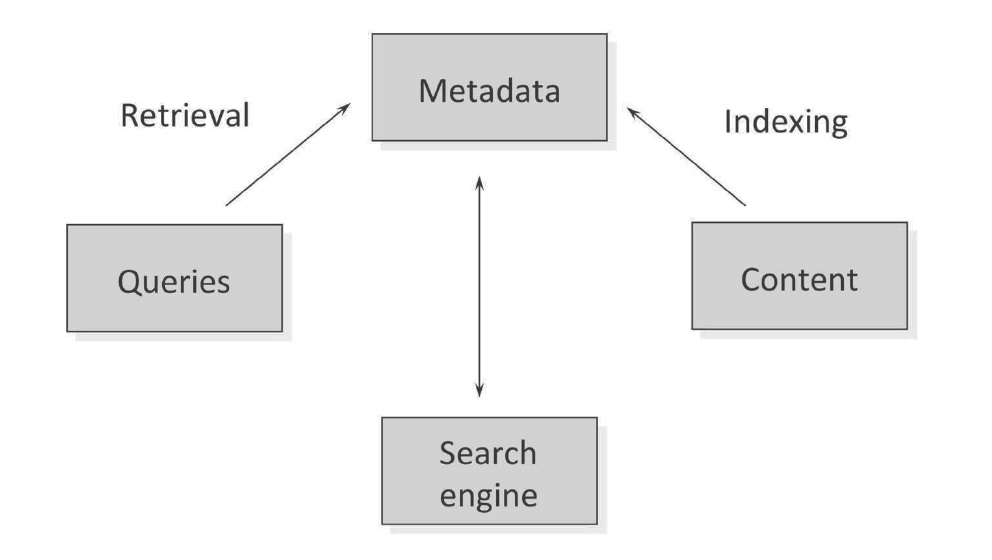
\includegraphics[width=\linewidth]{irprocess}
	\caption{Basis of Information Retrieval (IR) process.}
	\label{fig:1}
\end{figure}

The intelligent portal is built on top of the Figure \ref{fig:1}, which depicts a high-level perspective of the IR process. A person's information requirements to retrieve the \textit{content} is the primary focus of the IR process. The first step is to ask the IR system a \textit{query}. Metadata is used by \textit{search-engine} to match a user's query with relevant material. In IR, there are two types of thinking. Metadata are assigned to content objects during the \textit{indexing} process; \textit{retrieval} occurs when a user does a search and receives the results of that query \citep{prob2}.

\section{Intelligent Chatbot}

In the last decade, individuals have turned more and more to chatbot technology for help with things like social and emotional support and finding information \citep{chat1}. Chatbots, also known as conversational interfaces, allow computers to engage with humans in a more natural way \citep{chat2}. Conversation agents, dialogue assistants, and intelligent virtual assistants are all names for chatbots. Although chatbots have gained popularity among academics, developers, and end users, little is known about how well they can assist those living with dementia (which includes Alzheimer's disease and associated dementias) or those who care for them. This research also fills the knowledge gap by conducting a comprehensive assessment on available chatbots with a dementia emphasis.

A new research found that although AI chatbots show promise in helping dementia patients and aiding carers, the technology still has a long way to go before it is genuinely effective and dependable \citep{chat3}. Six chatbots were included in the study, and the researchers used an evidence-based evaluation technique to evaluate the quality and breadth of each. The chatbots were evaluated based on how well they might aid those with dementia and their caretakers. Five of the bots were voice-activated Alexa Skills, while the sixth was a smartphone app that only communicated through text. Some applications were made to assist patients remember things, while others were made to teach others about dementia. The applications were graded on how well they performed, how useful they were, how they made people feel, how happy they made them, how satisfied they made them, and how ethically they behaved.

\section{Aim and Objectives}
Long-term carers of persons with dementia may find it difficult, to access essential information and support. There are no such intelligent portal which might be helpful for the better care support in the field of dementia. When categorising the technologies, it is needed to take into account who would be the primary customers and benefactors of each one, where they would be located in the care environment, and how advanced their dementia was. The aim of this research is to develop a novel data driven intelligent information and resource portal based on the specific needs of the caregiver to any given situation. And, the objective refers to application of intelligent information retrieval methods coupled with current real-world data on resources and services to direct the right information for each contextualized query. The resource portal should be more intelligent that can reflect AI knowledge. An intelligent chatbot can be functioned adequately to help user with their queries, since they were not too difficult to master for the average user. 

The aim of this dissertation is to develop an intelligent resource portal for caregivers to help with people who have dementia. The associated objectives are:
\begin{enumerate}[label=\arabic*)]
	\item To study the relevant literature review and related works.
	\item To collect and gather required informations and resources regarding the dementia people. 
	\item To design and implement an intelligent portal with essential features.
	\item To test the developed system with collected data and helpful information.
\end{enumerate}

The purpose of this study is to accommodate for the distinct physical and cognitive deficiencies of dementia patients while also reducing carers stress with the help of artificial intelligence. In the health care and medical fields, the idea of information portals is not new, and there are a number of portals that give access to information and services on a wide range of health-related topics \citep{am1}. To suit the demands of individual users, more and more portals are being created to offer an intelligent interaction among consumers and relevant information resources. There are a slew of cutting-edge health care portals accessible right now. WebMD and HealthCentral.com are two healthcare websites with searchable healthcare information. Access to the portal may be customised based on the user's preferences, requirement, level of security, and accessible authorisation \citep{am2}. The research will help to build a intelligent information portal for the caregiving of people who have dementia.

\goodbreak

\section{Structure of Dissertation}
The rest of the dissertation structure will emphasize on:

\begin{enumerate}[label=$\ast$]
	\item Literature review - This section will highlight all the literature work related to the topic. It will also focus on the chatbot technology on health. Natural Language Processing and IR methods will also be reviewed here.
	\item Analysis - In this part, it will go through the proposed solution and software development process. All necessary software and hardware components, both internal and external, are listed. The project timeline and expected completion dates for each milestone will be shown graphically using a Gantt chart.
	\item Design - In this part, it will showcase web portal's overarching design, complete with user interface (UI) designs and storyboards that lay out the GUI in great detail. A visual representation of the technological architecture, such an activity diagram, will be created and presented. It will explain the interplay between all of the parts. Database structure and connections will be presented.
	\item Implementation and Testing - This section will detail the steps used in creating the solution's implementation. Unit testing and relevant test cases will be used to validate the chatbot and other features after development is complete. If any problems are found, they will be addressed to achieve the highest possible standard.
	\item Evaluation - The finished product is going to be assessed in order to establish both its level of quality and its overall worth. It will go into depth on the process that was used to build the entire project. When thinking back on the experience as a whole, it's important to point out both the aspects of the project that went particularly well and the ones that may need some tweaking for the future.
\end{enumerate}

\goodbreak
   


\def\baselinestretch{1.66}
\medskip


%%% ----------------------------------------------------------------------

% ------------------------------------------------------------------------
% -*-TeX-*- -*-Hard-*- Smart Wrapping
% ------------------------------------------------------------------------
\def\baselinestretch{1}

\chapter{Literature Review}

\def\baselinestretch{1.44}

%%% ----------------------------------------------------------------------

This chapter reviews the related literature work in the field of dementia care, as well as looks over chatbot technology in healthcare and natural language processing with knowledge base for my dissertation topic. 
   
\smallskip

%%% ----------------------------------------------------------------------
\goodbreak
\section{Related Work on Dementia}
People with dementia and their caregivers are becoming more interested in creating and testing technology that might enhance their quality of life and care. The Family Caregiving Institute hosted a Research Priorities in Caregiving Summit: Advancing Family-Centered Care Across the Serious Illness Spectrum in 2018. "Evaluate technologies that promote choice and collaborative decision making" and "identify where technology is best incorporated throughout the trajectory of caring" are the first two research goals listed \citep{three}. Such a technological breakthrough might have a significant impact on the field of dementia care. There are several explanations for this. 

Firstly, Delaying or averting its need for brief care in the rapidly ageing population is a first step in alleviating the pressure on public funds and ensuring the viability of institutional services amid a quickly expanding senior group \citep{lit1}. Secondly, another benefit of a large-scale deployment of robotics-assisted care is that it might minimise the load on unpaid carers while also improving quality of care due to a decline in the ratio of caregivers to patients \citep{int1}. Thirdly, and without any viable treatment options in sight, big data platforms can uncover insights from enormous volumes of unstructured data and enhance prevention, diagnosis and therapy and care administration \citep{lit2}. Finally, even more importantly, artificial intelligence (AI) is a powerful tool that may be used to enhance the delivery of patient-centered healthcare solutions that are tailored to an individual's needs \citep{lit3}. In addition to helping patients fulfil their desires, this would empower them and enhance their quality of life. 

According to previous studies, persons with dementia may utilize a variety of technologies tailored to their requirements, such as computers \citep{four} and touchscreen devices \citep{five}. Likewise, efforts to build technology-based therapies for dementia carers have increased during the past decade \citep{six}. There are also an increasing number of smartphone applications that cater to the requirements of dementia patients and/or carers \citep{seven}. Cognitive therapies using computers were shown to be more effective than noncomputer-based ones in enhancing cognition in adults with dementia, according to the systematic review by \cite{four}. For dementia caregivers, the effectiveness of technology-based therapies in enhancing psychosocial outcomes was widely observed, but not in increasing caring skills or care self-efficacy, according to a systematic evaluation of these programmes. Patients with dementia and their carers really aren't well-versed in the usage of chatbots \citep{six}.

\section{Chatbot Technology and Health}

Websites, smartphones (like Siri), applications for smartphones and tablets, SMS texting, and even smart home devices (like Alexa) may all be used to run chatbots. It was determined by \cite{lit.ch1} that chatbots may take one of three routes in handling conversations: There are three main types of chatbots: (1) finite state, where the user is guided through a set sequence of dialogue steps; (2) frame based, in which the chatbot starts asking questions and the user's answers assist the chatbot through an unstructured flow of communication; and (3) agent based, in which artificial intelligence enables the chatbot and user to interact through sophisticated conversation. According to the same evaluation, chatbot software may let the platform or the individual user take the lead in a conversation, which may take place either in written or spoken form.

Despite chatbots' widespread application in fields as diverse as customer service, education, website user support, and entertainment, researchers have recently discovered that they may also serve important roles in health care \citep{lit.ch2}, particularly in symptom self-assessment and telemedicine \citep{lit.ch3}. A variety of chatbots have been created and tested to help with issues in health care, such as those related to HIV/AIDS \citep{lit.ch4}, drug misuse and mental health assessment \citep{lit.ch5}, and weight management \citep{lit.ch6}. So far, studies using chatbots in the medical field have shown encouraging outcomes. Psychotherapy and self-cohesion to treatment are two areas where chatbots have been shown to be helpful in an evaluation of their use in psychiatric care \citep{lit.ch7}.

Using chatbots in healthcare has been shown to be beneficial for both patients and healthcare systems. Patients may benefit from the use of chatbots for a variety of reasons, including assistance with therapy management and encouragement at difficult times \citep{lit.ch8}. Telehealth systems may save money and enhance patient outcomes by deploying well-designed chatbots for data collection, education, engagement, and resource allocation \citep{lit.ch3}. \citet{lit.ch1} recently conducted a comprehensive review on the topic and found that despite the promising future of conversational bots in healthcare, only a small amount of research has been conducted on the topic.

\section{Natural Language Processing and Knowledge Base}
It is generally agreed upon that the chatbot engine, also known as the Natural Language Understanding (NLU) engine, is one of the most essential components of a chatbot \citep{lit.kn1}. The Natural Language Understanding (NLU) is responsible for the translation of conversational dialogues into actions that can be comprehended by the computer. In order to comprehend the natural language utilised in interactive user interfaces such as chatbots, NLU engines make use of a wide range of artificial intelligence (AI) techniques. Machine Learning (ML) and Natural Language Processing (NLP) are the two techniques that make up these methodologies \citep{lit.kn1}. The chatbot's ability to understand the context of a user's message is crucial for responding to questions and resolving issues it would otherwise be unable to handle. This is because the user input is ambiguous or might be interpreted in several ways. So when context is retrieved as well as the proper intent is coupled to carry out the intended action for the user, the chatbot is said to have the ability to maintain its state, which is also known as the quantity of user provided input (utterances). Conversational interfaces rely heavily on intents.

It is common for knowledge-based systems to comply with the principles of developing a knowledge base, constructing an inductive reasoning, and a method for user engagement. In order to create computational inference rules that closely approximate human thinking, such solutions need the involvement of subject matter experts in the relevant fields. In an effort to better understand the course of multiple sclerosis, \cite{lit4} built a fuzzy logic-based decision system. Language variables, values, and membership functions were used to quantify the domain knowledge and portray it with the help of clinical professionals. A metaheuristic optimization model was then used to find the maximum possible rate of proper categorization for the healthcare stance process, which was then codified into if-else rules \citep{lit4}. Meningitis diagnostics may be aided by a system that uses a graphical model to express domain knowledge and fuzzy interactions between ideas \citep{lit5}.

\section{Online Discussion Forum on Healthcare}
Back in the day, when the internet was still young, a significant amount of study was conducted to determine how'safe' the health information that was readily accessible was. In spite of persistent worries, researchers discovered minimal levels of reported injury \citep{lit.fo1}. As social media became more popular, the goals of research switched to investigate how people were utilising Internet discussion boards \citep{lit.fo2}. The study came to the conclusion that contact with other people who had a similar health condition was essential for those who had such conditions \citep{lit.fo3}. They were aware of the need to evaluate the information that was being offered, despite the fact that people valued the expertise which others dealing with the same disease may contribute \citep{lit.fo4}. The recent study done by \cite{lit.fo5} shown that social media was extensively utilised by patients as well as carers, with a variety of sites and online forums being used to offer support for patients and caregivers.

People are encouraged to talk about their health on online discussion forums, and there is a forum for almost any imaginable health issue \citep{lit.fo6}. Many healthcare-related studies that use internet forums to collect data on patient experiences do so by doing retrospective or tertiary evaluations of archived postings, which prevents researchers from engaging in follow-up questioning \citep{lit.fo7, lit.fo8}. While more and more health researchers are using online discussion forums to obtain qualitative information from patients \citep{lit.fo9, lit.fo10}, few have examined how effective discussion platforms are for knowledge exchange and virtual communities among health professionals \citep{lit.fo12}.


\def\baselinestretch{1.66}
\medskip


%%% ----------------------------------------------------------------------

% ------------------------------------------------------------------------
% -*-TeX-*- -*-Hard-*- Smart Wrapping
% ------------------------------------------------------------------------
\def\baselinestretch{1}

\chapter{Analysis and Requirements Specification}

\def\baselinestretch{1.44}

%%% ----------------------------------------------------------------------

This chapter describes the details analysis and specification requirements for my dissertation project. 

\smallskip

%%% ----------------------------------------------------------------------
\goodbreak
\section{Proposed Solution}
Based on the findings of the literature analysis, it is clear that the healthcare industry is always looking for new ways to enhance customer service and boost service delivery via the use of cutting-edge technology. The proposed solution is to create a intelligent web portal that will
\begin{enumerate}[label=\arabic*)]
	\item show dementia related informations in categorized order,
	\item hold a chatbot in order to help users with their dementia related answers in a manner like a human conversation, 
	\item have a community forum to discuss about dementia related topics.
\end{enumerate}

The web portal will be routed to several pages which will show infromations about dementia, learning for dementia, technological solutions for dementia, and dementia related news and articles. The feasibility of incorporating a chat bot into applications has expanded as a result of developments in artificial intelligence, machine learning methods, higher aptitude for decision making, and a bigger availability of data. The user's question will be recognised and comprehended by the chatbot, and it will then come up with an acceptable answer depending on the overall context of the interaction. The portal will also connect the forum, where user will able to sign up, sign in, create post, and see the categorized posts.

\section{Information Collection}
This project is supported by Socitm (https://socitm.net/). Socitm is the UK’s leading
membership organisation of more than 2,500 digital and IT professionals helping shape and
deliver public services, with links to current work supporting people with dementia in Suffolk and Norfolk, the Building Research Establishment and a number of academic institutions. After meeting with them they provided initial requirements for the information related dementia care in the portal. As they didn’t have any kind of collected datasets, collecting information is one of the major tasks in this project. When someone in the family starts to suffer with dementia, then family members are totally unprepared, any support that one can find, any learning that exists and other people’s experiences and views are very valuable. Caregivers, be they professionals, family, friends etc. would benefit from a portal that contains: products, suppliers, and learning. These are the key area to be covered in the portal. 

There are many emerging technologies such as:
\begin{enumerate}[label=$\ast$]
	\item fall monitoring sensors
	\item community alarm systems that could be worn on the person (linked wirelessly) that were used for both monitoring and response in emergency
	\item door entry systems using voice, video, or both
	\item sensors linked to doors to make sure that the individual was moving around their home
	\item sensors linked to fridges, kettles, and other devices to monitor their use (and sometimes their contents)
	\item hearing loops
	\item at home medical support and diagnosis
	\item use of technology to keep people in touch with friends and relatives
	\item monitoring attendance in the home of external visitors including professionally sourced caregivers
	\item use of video within the home for safety and security although these technologies pose challenges in terms of privacy and appropriate use.
\end{enumerate}

The dataset is sort of collated information collected from background research and google search that: listed available technologies, who they might be available from, whether they had been used successfully (absence of review mechanisms), what costs there were, examples of best practice with balanced assessment of what had gone well/badly, ease of use, appropriateness, opportunities for collaborative approaches across both private and public sectors.

\section{Software Development Strategy}
It is essential to make a decision about a suitable methodology before beginning the advancement of any software programme. This will guarantee that a reasonable timetable is created for each step of the project and that needs are described in a concise manner. During the process of developing and designing this programme, a number of different development approaches will be examined and taken into consideration. As an offshoot of the waterfall model, incremental model of the software development methodologies came along. Design, development, and testing of the application all occur in incremental steps \citep{ana1}. Each build will culminate in the production of a new module or feature. 

\begin{figure}
	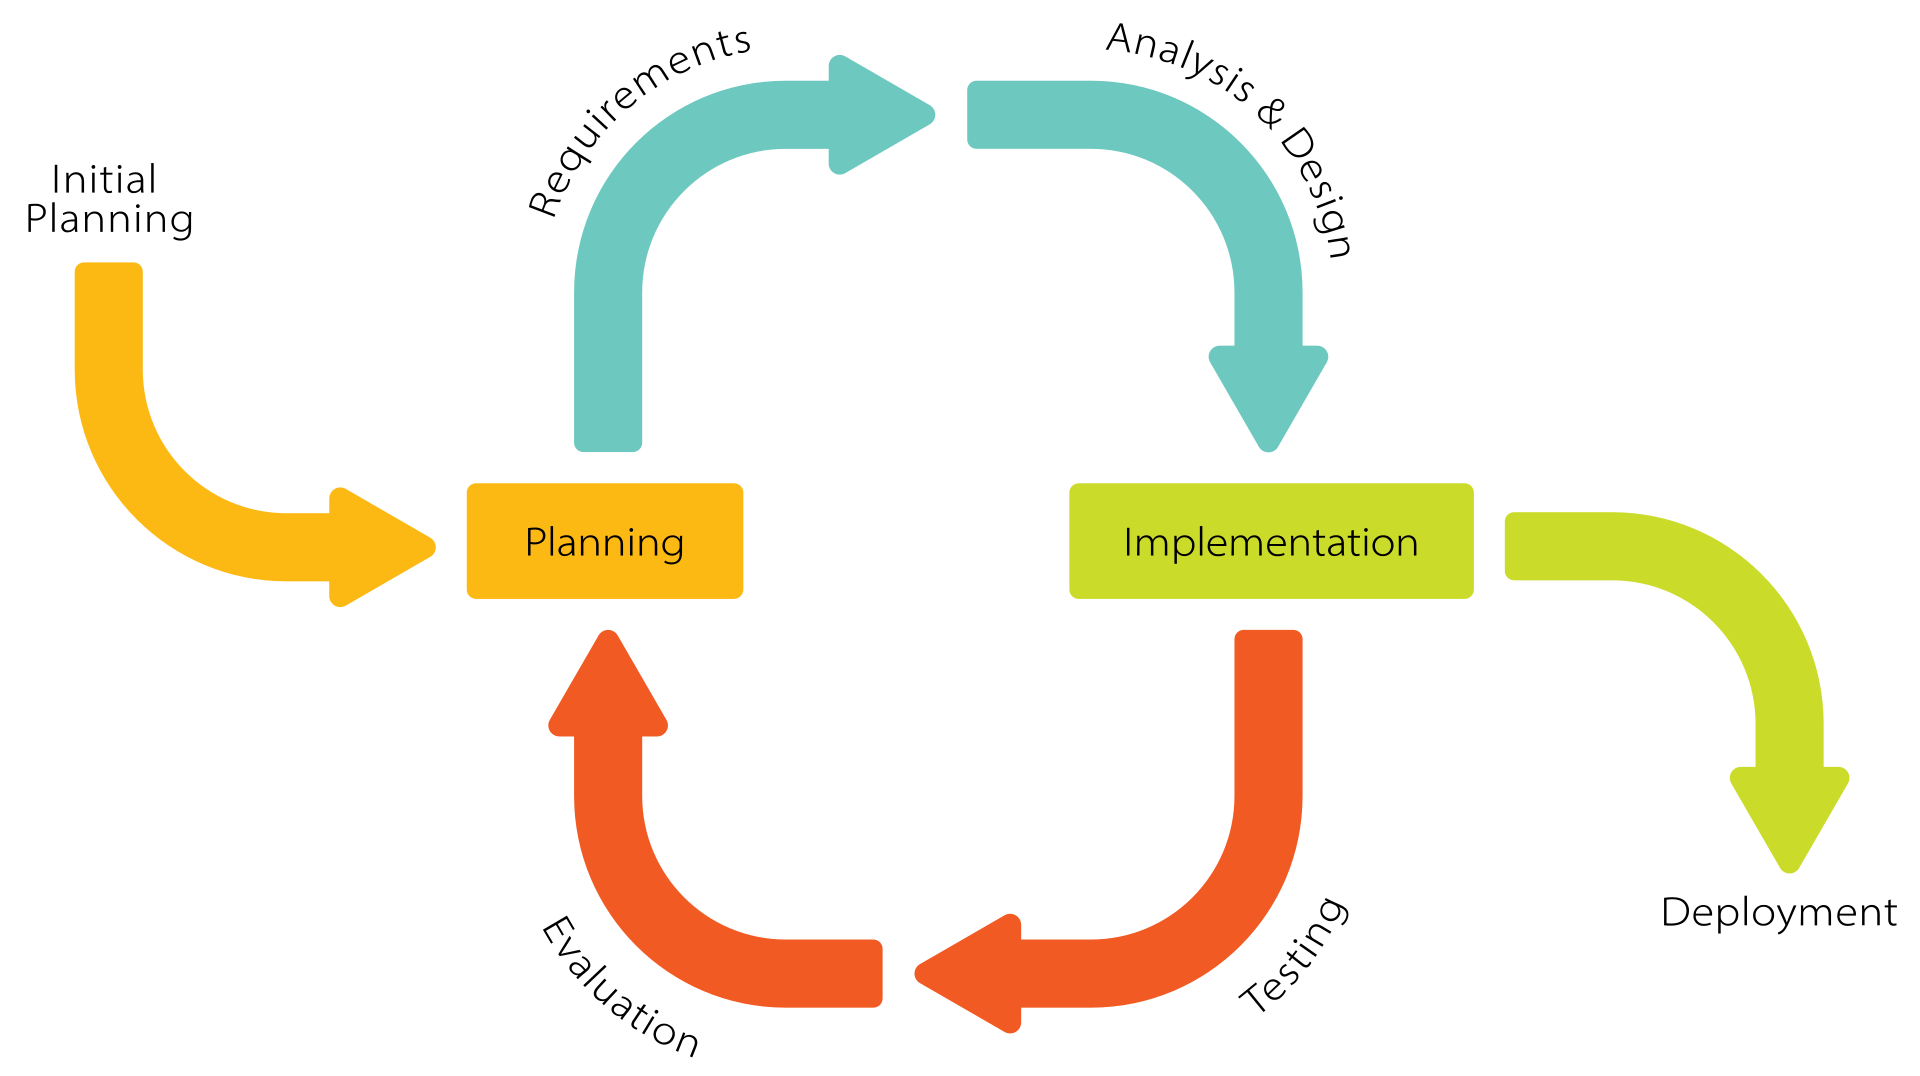
\includegraphics[width=\linewidth]{incremental}
	\caption{Incremental Model Overview.}
	\label{fig:2}
\end{figure}

Figure \ref{fig:2} displays the incremental model methodology. The project's complexity will increase as new needs are found and included into each incremental build, building on the features introduced in earlier versions. Early fault detection in brief cycles simplifies testing and troubleshooting. This project should use incremental development. Each successive build makes it straightforward to integrate new needs during the development process, making the incremental approach perfect for this project. 

\section{Software and Hardware Specifications}
Listed below are the software and hardware prerequisites that must be met in order to successfully build the web portal with chatbot and forum.
\subsection{Software Requirements}
\begin{enumerate}[label=$\bullet$]
	\item Operating System: Windows or Linux
	\item Front-end: HTML, CSS, Bootstrap, Javascript
	\item Back-end: Python
	\item Browser: Mozilla Firefox, Google Chrome
	\item Django
	\item Flask
	\item Visual Studio Code
	\item SQLite
	\item nltk
\end{enumerate}
\subsection{Hardware Requirements}
\begin{enumerate}[label=$\bullet$]
	\item Processor: Intel Core i3 (minimum) 
	\item Ram: 2 Gb (minimum)
	\item Hard drive: 50 Gb
\end{enumerate}

\section{Project Planning}

While a list of work progress outlining the project breakdown is created to serve as a management plan to be adhered to over the project lifespan, modest modifications may be made in each iteration as certain requirements may need to be modified. Project deliverables have their own individual checklists of tasks to be taken throughout each iteration. Create a Gantt chart outlining the semester-by-semester project activities and a risk management strategy.

\subsection{Project Milestones}
The project's progress is evaluated using the milestones, which also serves to establish due dates for activities and reveal which goals have been attained. Table \ref{table:1} highlights the project milestones.

\begin{table}[!h]
	\centering
	\begin{tabular}{ |c|c|c| } 
		\hline
		Milestone & Milestone Description & Completion Date \\
		\hline
		1 & Literature Review & 25.05.2022 \\ 
		2 & Analysis & 06.06.2022 \\ 
		3 & Design & 20.06.2022 \\ 
		4 & Iteration 1 & 01.07.2022 \\
		5 & Iteration 2 & 16.07.2022 \\
		6 & Iteration 3 & 27.07.2022 \\
		7 & Final Iteration & 08.08.2022 \\
		8 & Testing & 15.08.2022 \\
		9 & Evaluation & 21.08.2022 \\
		\hline
	\end{tabular}
	\caption{Project Milestones.}
	\label{table:1}
\end{table}

\subsection{Project Work Breakdown}
To ensure the project's success while using an incremental approach, it's crucial to define what features must be included throughout each iteration. In the event that new necessities emerge during development, they will be included into an ongoing iteration if they are manageable, or a new variant would be introduced to the schedule if they are substantial. Table \ref{table:1} shows the detailed iterations of the project.
\begin{table}[!h]
	\centering
	\begin{tabular}{|c|p{10cm}|} 
		\hline
		Iteration & Functional Implementation \\
		\hline
		Iteration 1 & \begin{itemize}[label=$\ast$] 
			\item Install and make a Django app
			\item Develop a homepage
			\item Develop four connecting pages
		\end{itemize} \\ 
		\hline
		Iteration 2 & \begin{enumerate}[label=$\ast$]
			\item Install and make flask app
			\item Make intent JSON file
			\item Train knowledge base model
			\item Implement standalone chatbot
			\item Enable cross-origin resource sharing
			\item Connect chatbot to the main site
		\end{enumerate} \\ 
		\hline
		Iteration 3 & \begin{enumerate}[label=$\ast$]
			\item Develop a forum  site
			\item Add sign in and sign out
			\item Implement create, delete, and update post
			\item Implement comment section
		\end{enumerate} \\ 
		\hline
		Final Iteration & \begin{enumerate}[label=$\ast$]
			\item Integrate forum to the main site
			\item Necessary bug fixing and update
		\end{enumerate} \\
		\hline
	\end{tabular}
	\caption{Project Iterations.}
	\label{table:2}
\end{table}

When each cycle has been completed, the final answer will have been produced. The project is going to be reviewed so that the lessons learned may be highlighted, and reflection will be done on the full project life cycle. This provides me with the chance to talk about what was accomplished as well as the processes or aspects of future projects that I would approach differently as a result of the lessons I learned from this experience.

\subsection{Risk Management}
A critical part of minimising the effects of potential hazards on a project's overall success is determining and controlling the risks and consequences connected with the project. Prevention measures may be implemented to reduce the possibility of a risk arising if its potential effects are known early in the project's development. Github will be used to back up code and avoid loss, individual initiative will be used to stay on top of the project plan, the project report and critical documents will be backed up on a regular basis, and if an unanticipated day off happens, the lost work will be made up for.

\subsection{Project Management}
A Gantt chart that was made in online gantt chart maker and displays the timetable for the project can be seen below in Figure \ref{fig:3}. It is possible to determine once the project milestones need to be finished by using Gantt charts, which helps ensure that the work is completed on time. The following chart provides a summary of the tasks, as well as the sequence that they are going to be contested and the amount of time allocated to each activity.

\begin{figure}[h!]
	\centering
	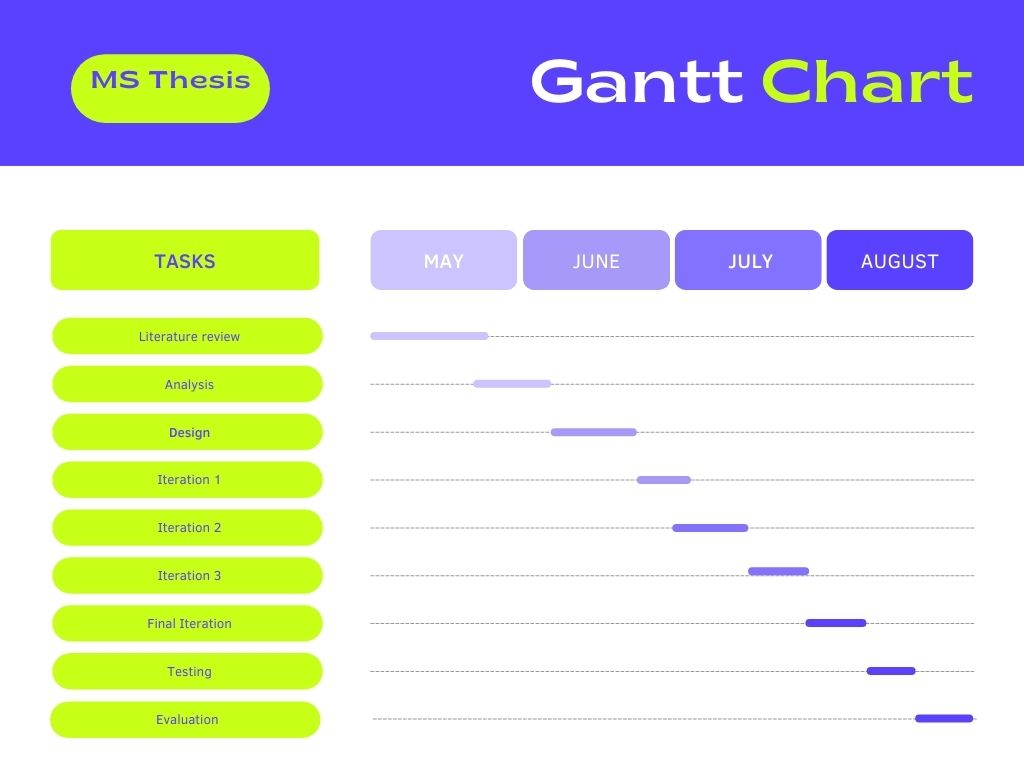
\includegraphics[width=0.8\textwidth]{gantt}
	\caption{Gantt chart for the project.}
	\label{fig:3}
\end{figure}

\def\baselinestretch{1.66}
\medskip

%%% ----------------------------------------------------------------------

% ------------------------------------------------------------------------
% -*-TeX-*- -*-Hard-*- Smart Wrapping
% ------------------------------------------------------------------------
\def\baselinestretch{1}

\chapter{Methodology Design}

\def\baselinestretch{1.44}

%%% ----------------------------------------------------------------------

This chapter describes the overall methodology design for my dissertation project, which include web portal design, chatbot design, and community forum design. 
   
\smallskip

%%% ----------------------------------------------------------------------
\goodbreak
\section{Web Portal}
The web portal have a base page as a homepage, then it connects to the other pages. User can be navigate through all the pages easily. The client side of the web application is developed using HTML, CSS, Bootstrap, Javascript, and Django framework. 

\subsection{Architectural Design}
The architecture of a website refers to the pages of the website organised in a hierarchical fashion. The internal connecting displays this structure in a clear and concise manner. Users of your website should be able to readily access the information they need, and the structure of your website should also assist search engine crawlers comprehend the connection between the various pages \citep{web}. You may improve the user experience of your website by designing it using a structure that has been used on the website. Even if you have the most excellent content in the world, visitors won't stick around if they can't locate what they're looking for on your website. The home page serves as the starting point for the structure of most websites, which takes the form of a rooted tree graph. The pages that have links leading out from the homepage are referred to as branches, and from that point forward, each page has further branches growing out of it. These branches ultimately connect to one another. 

Figure \ref{fig:4} illustrates the architectural design of the web portal. The website architecture here is very simple. The landing page is the homepage, which will hold all the summary information and the AI chatbot. AI chatbot will remain on the same position on the web portal all the time. From homepage other pages can be accessed by the navigation menu, description links, and html sitemap on footer. All the page will be simple and user can be moved back to homepage from any page. The linked pages includes:
\begin{enumerate}[label=\arabic*.]
	\item \textbf{About Dementia:} This page highlights the information and knowledge about dementia.
	\item \textbf{Dementia Learning:} This page displays the detailed learning for the dementia care.
	\item \textbf{Technologies in Dementia:} This page holds information regarding technological solutions for the dementia care.
	\item \textbf{Research \& News:} This page lists recent research and news regarding dementia.
	\item \textbf{Community Forum:} This page is the homepage of the community forum.
\end{enumerate}

\begin{figure}[!h]
	\centering
	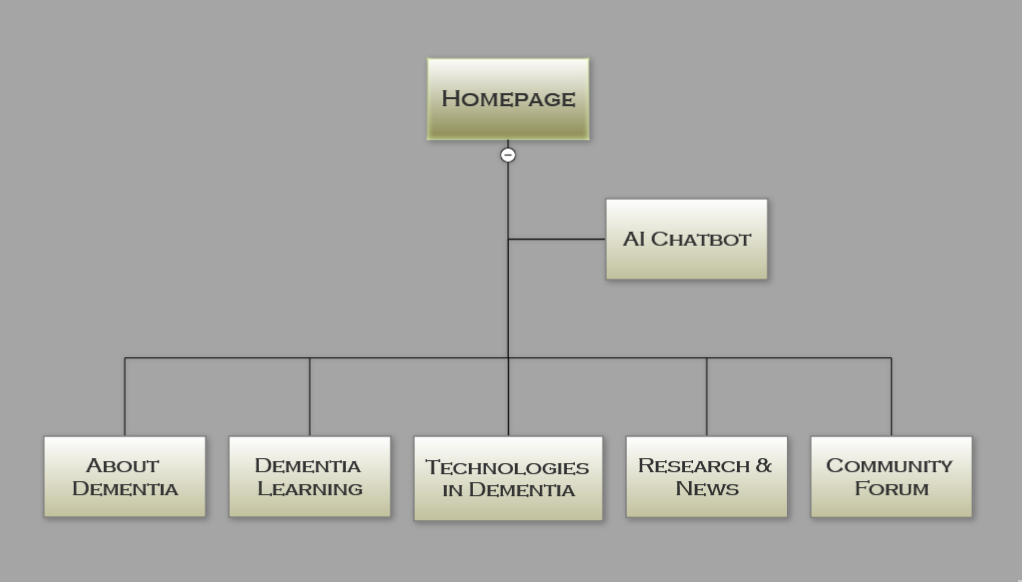
\includegraphics[width=\linewidth]{arch_design}
	\caption{Architectural design of the web portal.}
	\label{fig:4}
\end{figure}

\section{Chatbot}
The functionality of retrieval-based bots of an AI chatbot is built on the idea of oriented patterns or graphs. The bot is programmed to choose which of a limited number of prepared replies is the most appropriate to rank as the best response. The replies that are shown here are either keyed in by hand or are derived from a knowledge base that contains information that already exists. The client side of the chatbot is developed using HTML, CSS, Javascript, and Flask framework.

\subsection{Chatbot Concept}
The data is necessary for training my deep learning-based model, which I want to construct. However, given that this is a chatbot devoted to the subject of dementia, I will not be collecting or downloading any massive dataset. To train the model, I need just generate my own dataset. In order to make this datasets, I need to know exactly which intents I will be teaching. The "intent" of a user's interaction with a chatbot, or the motivation behind a user's communication to the chatbot, is what is meant by the term "intent." These intentions may differ from one chatbot solution to the next, depending on the domain for which I am creating the solution. Therefore, it is crucial that I learn the appropriate chatbot intentions as they pertain to the domain with which I will be interacting.

Understanding what users say or want to do is crucial for the chatbot's ability to respond appropriately, whether that's with a solution to a query, a search in a topic knowledge base, or any number of other activities. That's why it's crucial for the chatbot to read between the lines of user communications (to determine what the user means). The plan is to first determine the various intents that will be used, then create training data for those intents, and then train the chatbot model using the data from those training samples as model training data (X) and the intents themselves as model training categories (Y).

\subsubsection{Natural Language Toolkit (NLTK)}
With Python, NLTK is the go-to framework for manipulating human language data. Easy-to-use interfaces to more than 50 corpora and lexical resources like WordNet are included, as well as a set of text processing libraries for tasks like tokenization, classification, parsing, tagging, stemming, and semantic reasoning, as well as wrappers for commercial-grade NLP libraries and a lively community forum.

\subsubsection{TF-IDF}
Each document's TF-IDF (Term Frequency-Inverse Document Frequency) vectors will be calculated. This will produce a matrix in which each column has a different term from the introductory lexicon. The TF-IDF formula is the standard statistical approach for determining a word's importance inside a text. 

Phrase frequency, sometimes known as TF, refers to the number of times a certain term occurs in a particular text. IDF, which stands for "inverse document frequency," is a metric that determines the importance of a word inside a document by determining whether or not the word is used often across the whole text. According to the rationale behind the TF-IDF algorithm, the words that are used often in a text are less significant than the ones that are used seldom. The good news is that scikit-learn provides you with an in-built TfIdfVectorizer class that makes it very simple to generate the TF-IDF matrix.

\subsubsection{Cosine Similarity}
After obtaining the matrix, it is now simple for me to determine a score for the degree of resemblance. There are a few other approaches that may be used to do this, such as the Euclidean, Pearson, and cosine similarity scores. Once more the, there is no correct response to the question of which result is the best. I will be calculating a numerical amount that represents the similarities of the two words by using the cosine similarity, which is a statistical method. It is possible to make use of the cosine similarity score due to the fact that it is not reliant on the magnitude and may be calculated in a reasonably short amount of time (particularly when the scores of TF and IDF are taken into consideration).

\subsection{Workflow Diagram}
A step-by-step, linear depiction of a workflow from the beginning to the end is what is known as a workflow diagram. It illustrates how certain responsibilities, activities, or resources are distributed across several individuals or organisations. It also demonstrates the steps that need to be taken by your team in order to complete a job.

\begin{figure}[!h]
	\centering
	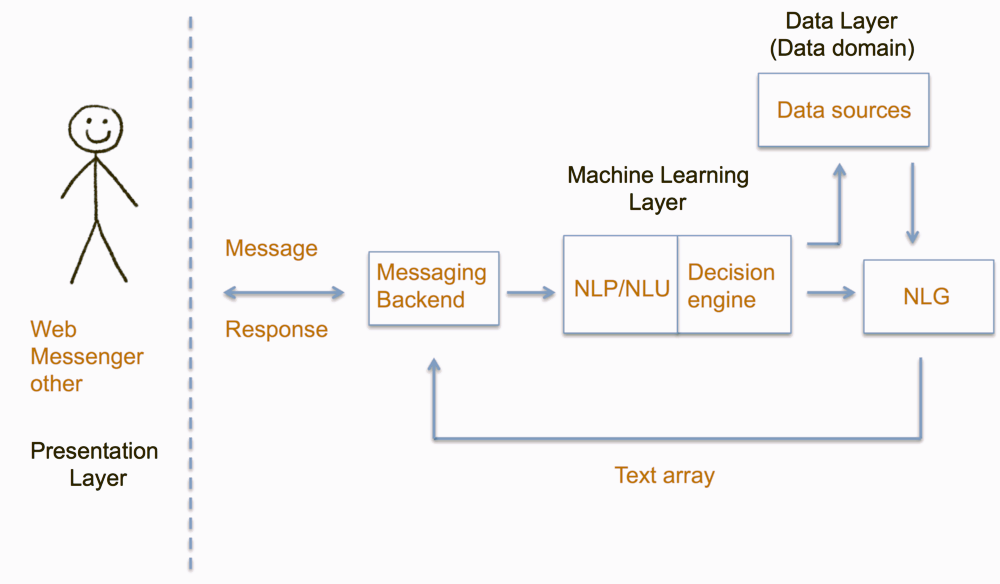
\includegraphics[width=\linewidth]{chatbot}
	\caption{Workflow diagram of the chatbot.}
	\label{fig:5}
\end{figure}

Figure \ref{fig:5} highlights the workflow of the intelligent chatbot. Here,
\begin{enumerate}[label=\arabic*)]
	\item The user poses inquiries to the chatbot, which are subsequently sent to the communication backend via the chatbot.
	\item Implementing natural language processing (also known as what occurs when computers understand language). Because NLP algorithms transform text into structured data, the computer must first translate such simple text request into instructions that it can understand.
	\item At this point, the chatbot will put this information into a decision engine, also known as a trained model, since, in the chatbot's head, it believes that it must fulfil a set of criteria in order to leave the conversational loop.
	\item The use of NLG, which refers to what takes place when computers compose language. NLG procedures take structured data and transform it into text, which is then returned to the user in a form that they can comprehend and relate to.
	\item This collection of user replies is sent back into the messaging backend, where it is processed and then delivered to the user in the form of a response.
\end{enumerate}

\section{Forum}
A community or discussion forum is an online gathering area where individuals may debate, exchange information, and chat to one other about a broad variety of things that they could be engaged in. HTML, CSS, Bootstrap, Javascript, and the Django framework are used to construct the client side of the group discussion forum. SQLite is the underlying technology for the database. 

The administrator is the one who is informed whenever an end-user submits an inquiry with the intention of obtaining information. The doubts subjects may be posted by any user, and any user can respond to the doubts of other users. There is one database in which all of the information is maintained, and that database is centralised. The user is able to post queries and invite other users to participate in Discussion. The database may be updated, but only the administrator has access to do so. This is great for a small workplace, school, or department, or really any organisation that is interested in successfully organising their space. There is a third kind of user known as a connected user who functions as an intermediate user and who, if they have the information, may also provide answers to queries posed by end users. Ability to publish articles and share resources, both of which may be read by users who have registered for the site. The end-user is responsible for making any necessary adjustments or updates whenever fresh data becomes available.

\subsection{Forum Modules}
The community forum includes six main modules, that made the interaction easier and users posts can be seen by everyone.
\begin{enumerate}[label=$\bullet$]
	\item \textbf{Category Module:} This is the primary section, where users may submit their inquiries by choosing a suitable category. Various users may provide responses to their inquiries.
	\item \textbf{Post Question Module:} This section is primarily for those who have already registered. The user is required to register in order for the Administrator to determine who is responsible for posting the questions. These registered people are the only ones who may submit a question in such a thorough way.
	\item \textbf{Registration Module:} The freshly entered user's information may be seen in more depth with the assistance of this module.
	\item \textbf{Comment Module:} Each and every question that is asked will receive an accurate response from the discussion forum staff, and in addition to that, they may get a lot of responses from a variety of different users.
	\item \textbf{Discover Module:} Here, visitors may respond to polls and quizzes. This module is useful for both registered and non-registered users. They may also check out the site for answers.
	\item \textbf{Search Module:} Users may enter their inquiries into this module, and the system will provide relevant results. Articles and innovations containing the search term are linked to in the results. Anyone, registered or not, may do a search.
\end{enumerate}

\subsection{Activity Diagram}
The activity diagram is crucial UML diagram for describing the system's state and behaviour across time. An activity diagram is a kind of flowchart that shows how one task leads to another. This is a system operation, therefore we may call it such. The direction of the flowchart is shown graphically, from one process to the next. This progression may be linear, branching, or concurrent. Using symbols like forks, joins, and others, activity diagrams may represent any kind of branching or branch-and-boundary relationships between two or more flows. Figure \ref{fig:6} shows the activity diagram for the community forum.

\begin{figure}
	\centering
	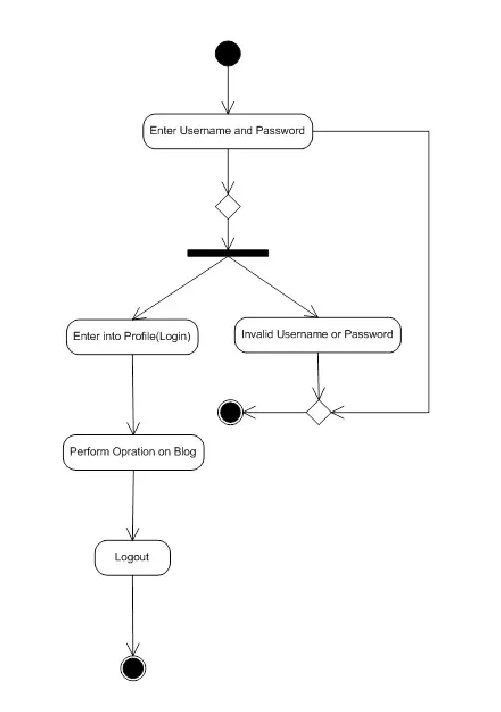
\includegraphics[width=\textwidth]{activity}
	\caption{Activity diagram of the community forum.}
	\label{fig:6}
\end{figure}

\subsection{Use Case Diagram}
Use case diagrams, which are more often known as behaviour diagrams, are used to represent a collection of activities (use cases) that some system or systems (the topic) should or can do in conjunction with one or more users who are not internal to the system (actors). Every use case has to provide some measurable and actionable outcome to the system's actors and other stakeholders in order to be considered successful. Figure \ref{fig:7} illustrates the use case diagram of the community forum.

\begin{figure}[!h]
	\centering
	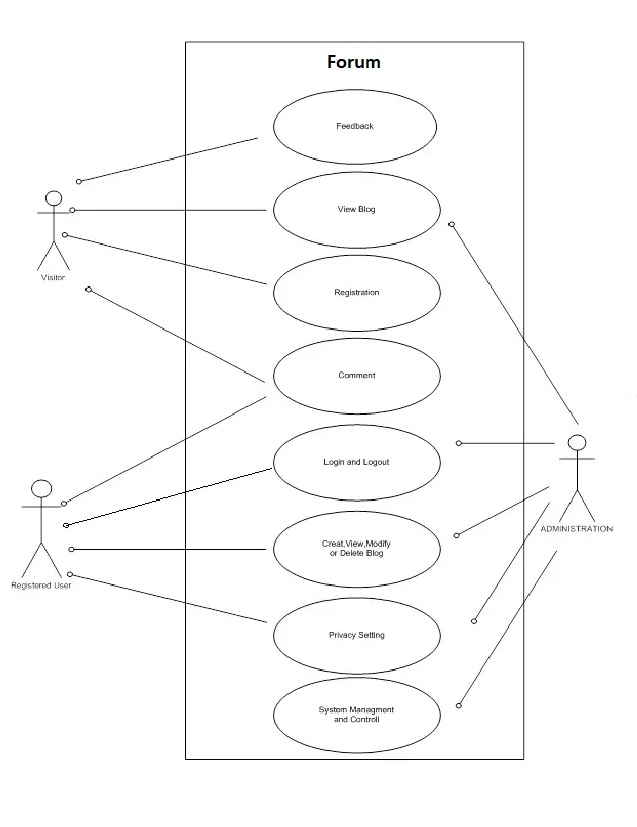
\includegraphics[width=0.8\linewidth]{usecase}
	\caption{Use case diagram of the community forum.}
	\label{fig:7}
\end{figure}

\subsection{Database Design}
Any programme that is designed absolutely needs a database architecture, but data store projects need it much more than other applications. Here, in the forum includes storing the information in the table according to authors, posts, categories, comments, and replies; it is essential that the table be managed in the appropriate manner. The login table for this forum is intended to be one of a kind in that it will only take one username at a time, and both the username and the password should have a length that is larger than zero. Figure \ref{fig:8} shows the database structure design for the forum that includes comprehensive listing of all of the tables and the fields.

\begin{figure}[!h]
	\centering
	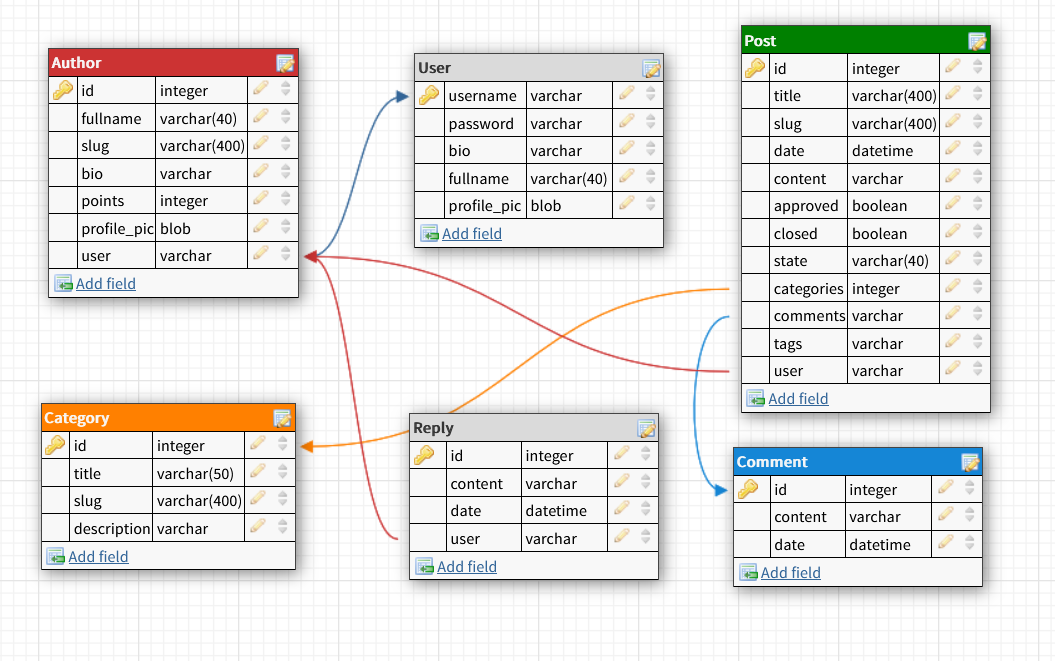
\includegraphics[width=\linewidth]{database}
	\caption{Schema diagram of the database for community forum.}
	\label{fig:8}
\end{figure}

\def\baselinestretch{1.66}
\medskip

%%% ----------------------------------------------------------------------

% ------------------------------------------------------------------------
% -*-TeX-*- -*-Hard-*- Smart Wrapping
% ------------------------------------------------------------------------
\def\baselinestretch{1}

\chapter{Implementation and Testing}
This chapter describes the detailed implementation and testing for my dissertation project.

\section{Implementation}
The main web portal is implemented using incremental approach. The main web portal and forum is built on Django app and the chatbot is built on Flask app. Finally, chatbot is integrated into web portal using cross-origin  resource sharing (CORS).

\subsection{Chatbot Development}

\subsubsection{Libraries and Packages}
The following is a list of the necessary Python packages.
\begin{enumerate}[label=\arabic*.]
	\item tensorflow==2.3.1
	\item nltk==3.5
	\item colorama==0.4.3
	\item numpy==1.18.5
	\item scikit\_learn==0.23.2
	\item Flask==1.1.2
\end{enumerate}

After that, importing all of the required library files are done. There are several libraries, such as:
\begin{enumerate}[label=$\ast$]
	\item nltk (Natural Language Toolkit), that provides many instruments for enhancing text and making it suitable for deep learning algorithms.
	\item json, is a Python module that loads json files straight into the language.
	\item pickle, is an application that loads pickle files.
	\item numpy, which is able to carry out operations in linear algebra in a highly efficient manner.
	\item keras, is the name of the framework for deep learning that can be utilised for training model.
\end{enumerate} 

\subsubsection{Initializing Chatbot Training}
At this point, it is time to begin the process of initialising all of the lists that will be used to hold my natural language data. There is the JSON file that I described previously, which is where the "intents" are stored. The following Figure \ref{fig:9} is a sample of what a typical JSON file truly looks like in its entirety:
\begin{figure}[!h]
	\centering
	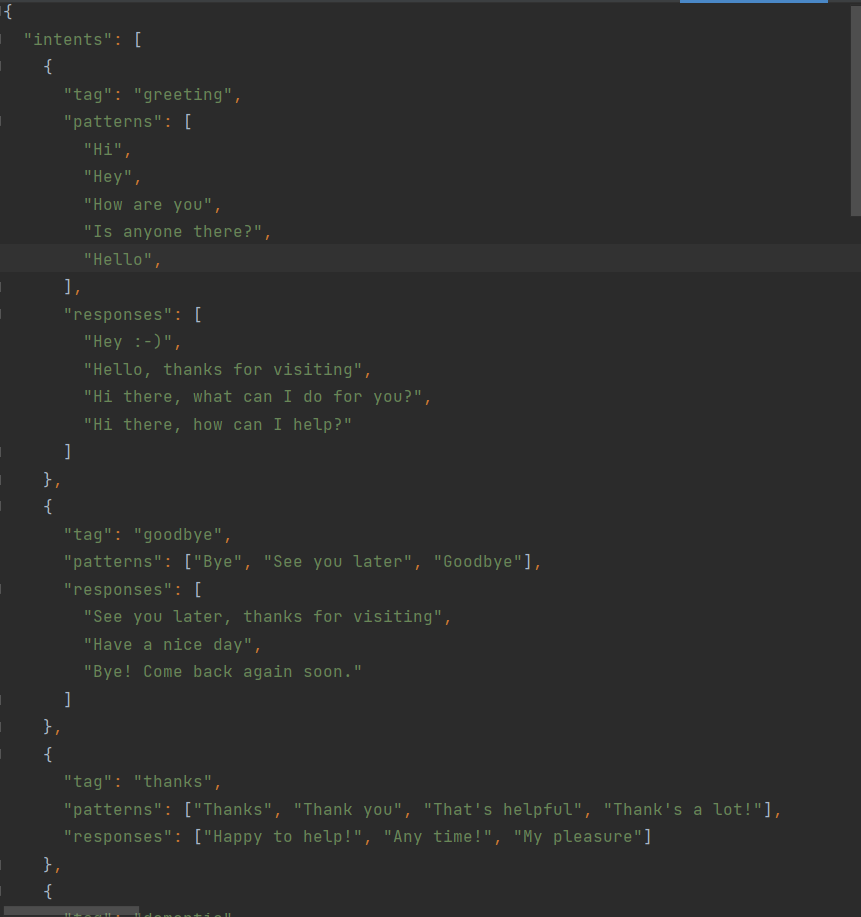
\includegraphics[width=0.8\textwidth]{intent}
	\caption{Simple JSON format.}
	\label{fig:9}
\end{figure}

To load the file, I make use of the json module, and then I store the loaded data to the variable intentions. There are sub-objects included inside the objects themselves. For instance, "patterns" is a property that falls within the category of "intents." Therefore, in order to extract all of the words included inside "patterns," I make use of a nested for loop to do so, and then I add those words to my list of words. The next thing I do is add each pair of patterns to my documents list inside the tag that corresponds to them. I also put the tags into the classes list, and to prevent them from being repeated, I utilise a simple conditional expression.

After that, I take the list of terms and lowercase and lemmatize all of the words that are included inside it. In the event that you were unaware, "lemmatize" is the process of reducing a word to its essential meaning, also known as its lemma. For instance, the phrases "walking," "walked," and "walks" all derive from the base word "walk," which is simply referred to as "walk." Lemmatizing the language serves the objective of reducing everything to the most fundamental level it can possibly be reduced to. When I really analyse these phrases for machine learning, it'll save a lot of time and save me from making errors that aren't essential. This is somewhat similar to the process of stemming, which involves reducing a conjugated word down itself to base form, also known as the root form.

\subsubsection{Building the Deep Learning Model}
Let's set up a training data variable and fill it with some sample information. For each document, I am creating a large nested list with sacks of words within. The output row feature I have only serves as a key to the collection. Next, I do a train-test-split with the patterns serving as the X value and the intentions serving as the Y variable. Now that both our training and test data are prepared, we can go on to the next step of using a deep-learning model from keras that is called Sequential. The following Figure \ref{fig:10} describes the architecture of the model.

\begin{figure}[!h]
	\centering
	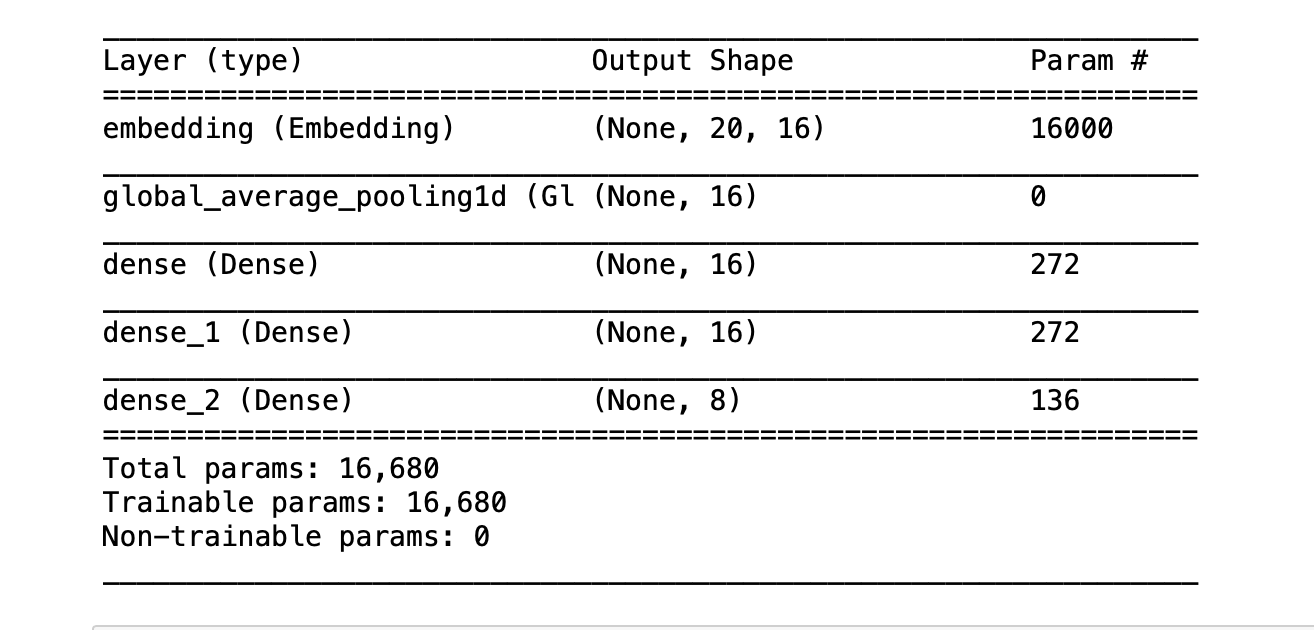
\includegraphics[width=\textwidth]{deeplearning}
	\caption{Sequential Model architecture.}
	\label{fig:10}
\end{figure}

A multi-layer perceptron is one of the simplest types of neural networks, and the Sequential model in keras implements this kind of network. The specific network in question is composed of three layers, the first of which has 128 neurons, the second of which contains 64 neurons, and the third of which contains the same quantity of intents as the amount of neurons. Keep in mind that the purpose of this network is to develop the ability to choose which intent to select given a set of inputs. Stochastic gradient descent, another very hard subject, will be used to train the model in order to improve its accuracy. When compared to traditional gradient descent, stochastic gradient descent performs more effectively. After the training of the model is complete, the whole thing is converted into a numpy array and the file is named chatbot model.h5.

\subsection{Website \& Forum Development}
The Table \ref{table:3} offers a convenient reference for the essential commands that need to run in order to begin the Django development process. Table \ref{table:4} on Appendix lists all the required dependencies for the website development.
\begin{table}[!h]
	\centering
	\begin{tabular}{ |c|c|c| } 
		\hline
		Description & Command \\
		\hline
		Setting up a virtual environment & python -m venv env \\
		\hline
		Activating the virtual environment & source env/bin/activate \\ 
		\hline
		Installing Django & python -m pip install django \\ 
		\hline
		Linking dependencies to install & python -m pip freeze $<$ requirements.txt \\
		\hline
		Setting up a Django Project & django-admin startproject $<$projectname$>$ \\
		\hline
		Starting a Django app & python manage.py startapp $<$appname$>$ \\
		\hline
		Running a Django server & python manage.py runserver \\
		\hline
		Creating migrations for database & python manage.py makemigrations \\
		\hline
		Applying migrations for database & python manage.py migrate \\
		\hline
	\end{tabular}
	\caption{Required Commands.}
	\label{table:3}
\end{table}

After developing main website, the forum is developed and all the features of the forum implemented. The community forum is connected to the the main site. the AI chatbot is integrated with the main site. Deployment is the most important step in the process of developing a successful system and instilling trust in the users that the new system will be both practical and efficient.

The installation of an updated version of an application to take the place of an existing one. It shouldn't be too difficult to manage a dialogue of this kind, provided there aren't any significant modifications to the system. Each individual programme is put through its own set of tests at the stage of development using the data. These tests ensure that the programmes are linked together in the manner that was outlined in the program's specification. Additionally, the user's satisfaction with the software system and its surrounding environment is ensured. The user has validated their acceptance of the system which has been designed and declared it to be acceptable. As a result, the platform is to be put into place really quickly. The user is provided with a straightforward operating process in order for them to comprehend the many tasks in a concise and expedient manner.

Initially as a first step the executable form of the application is to be created and loaded in the common server machine which is accessible to all the user and the server is to be connected to a network. The final stage is to document the entire system which provides components and the operating procedures of the system.

\section{Testing}
Testing is an essential stage in the lifecycle of every software development project. It should come as no surprise that when evaluating the limitations of the programme, specific faults and mistakes are discovered and recorded by means of test cases. Both the quality of the user experience and the general standard quality of the website and chatbot will both improve as a result of this change.

\subsection{Unit Testing}
The testing at the procedure level is performed initially. By providing incorrect inputs, the mistakes that have occurred may be identified and remedied. After that, testing at the level of the web form is performed. As an example, the proper storing of data inside the table. The dates have been input incorrectly and verified for accuracy. Incorrect email address and URL (Universal Resource Locator) for the website were provided and verified.

\subsection{Integration Testing}
Testing is performed on each individual module. The modules are then combined, and the finished system is tested using the test data, which has been specifically created to demonstrate that the functionality of the system correctly in all of its features and situations. Therefore, the system testing serves both as a validation that everything is in the right place and a chance to demonstrate to the user that the system is functional.

\subsection{Validation Testing}
Validation testing, which examines whether or not the programme functions as the user intended it to, is the last phase in the process. The end user, not the system developer, is the one who runs this test. This test, which is part of a procedure known as "Alpha and Beta Testing," is used by the majority of software developers to discover issues in which only the end user is able to identify. The successful completion of the whole project is dependent on ensuring that all of the end users are happy with it. There are a few different kinds of validation tests carried out on the project. In the registration form, the user's email address, phone number, and any other essential entries are checked for accuracy.

\subsection{User Testing of Chatbot}
It is chosen to conduct user testing across two channels of communication; Google Assistant and the AI Chatbot. This provides a glimpse into the genuine quality and overall utility of the chatbot, both of which are determined by the interaction experience that the user has with the chatbot. A series of questions designed to assess the chatbot's functionality were compiled in order to facilitate user testing. Several bugs is found on this testing, and those were solved accordingly. User can be experience issues regarding wrong answers twice in a 100 times. This can be solved training the model with different neural networks and more data. The process of putting a feature, or prototype through user testing involves soliciting feedback from actual end users as well as paying attention to consumers.

\goodbreak
\goodbreak
\section{Some Screenshots}

\begin{figure}[!h]
	\centering
	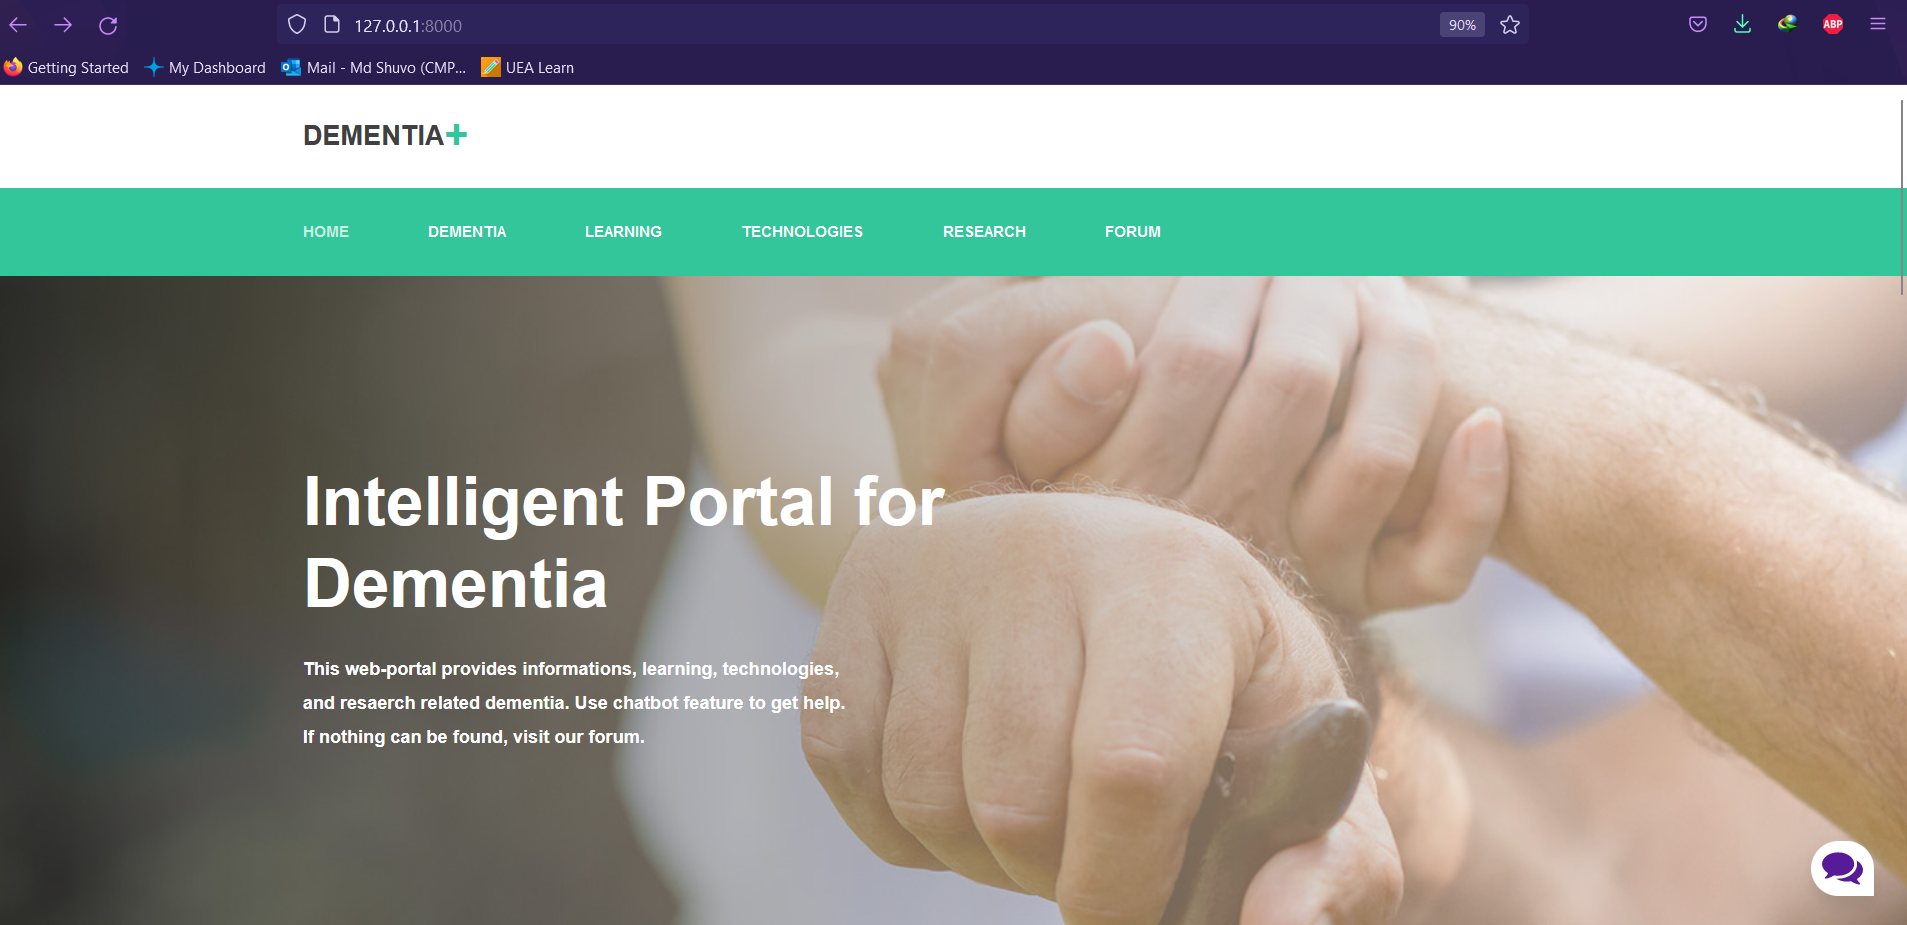
\includegraphics[width=0.85\textwidth]{homepage}
	\caption{Web portal homepage.}
	\label{fig:11}
\end{figure}

\begin{figure}[!h]
	\centering
	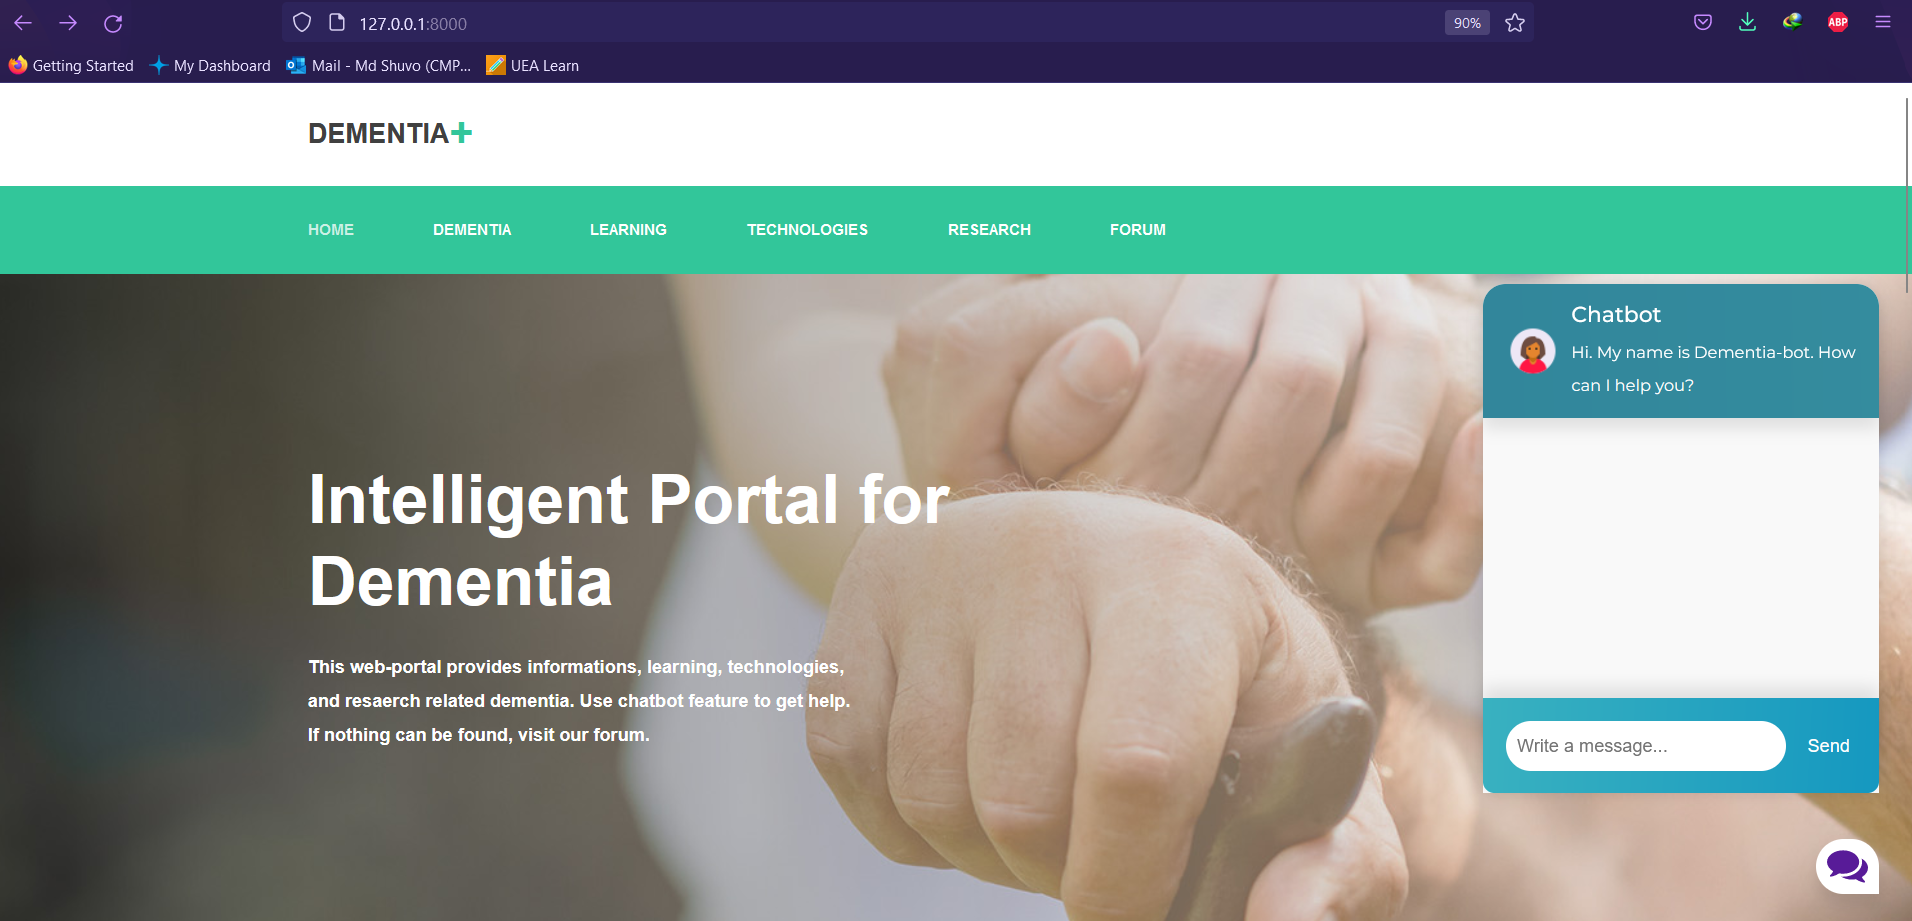
\includegraphics[width=0.85\textwidth]{home1}
	\caption{Homepage with chatbot opened.}
	\label{fig:12}
\end{figure}

\begin{figure}[!h]
	\centering
	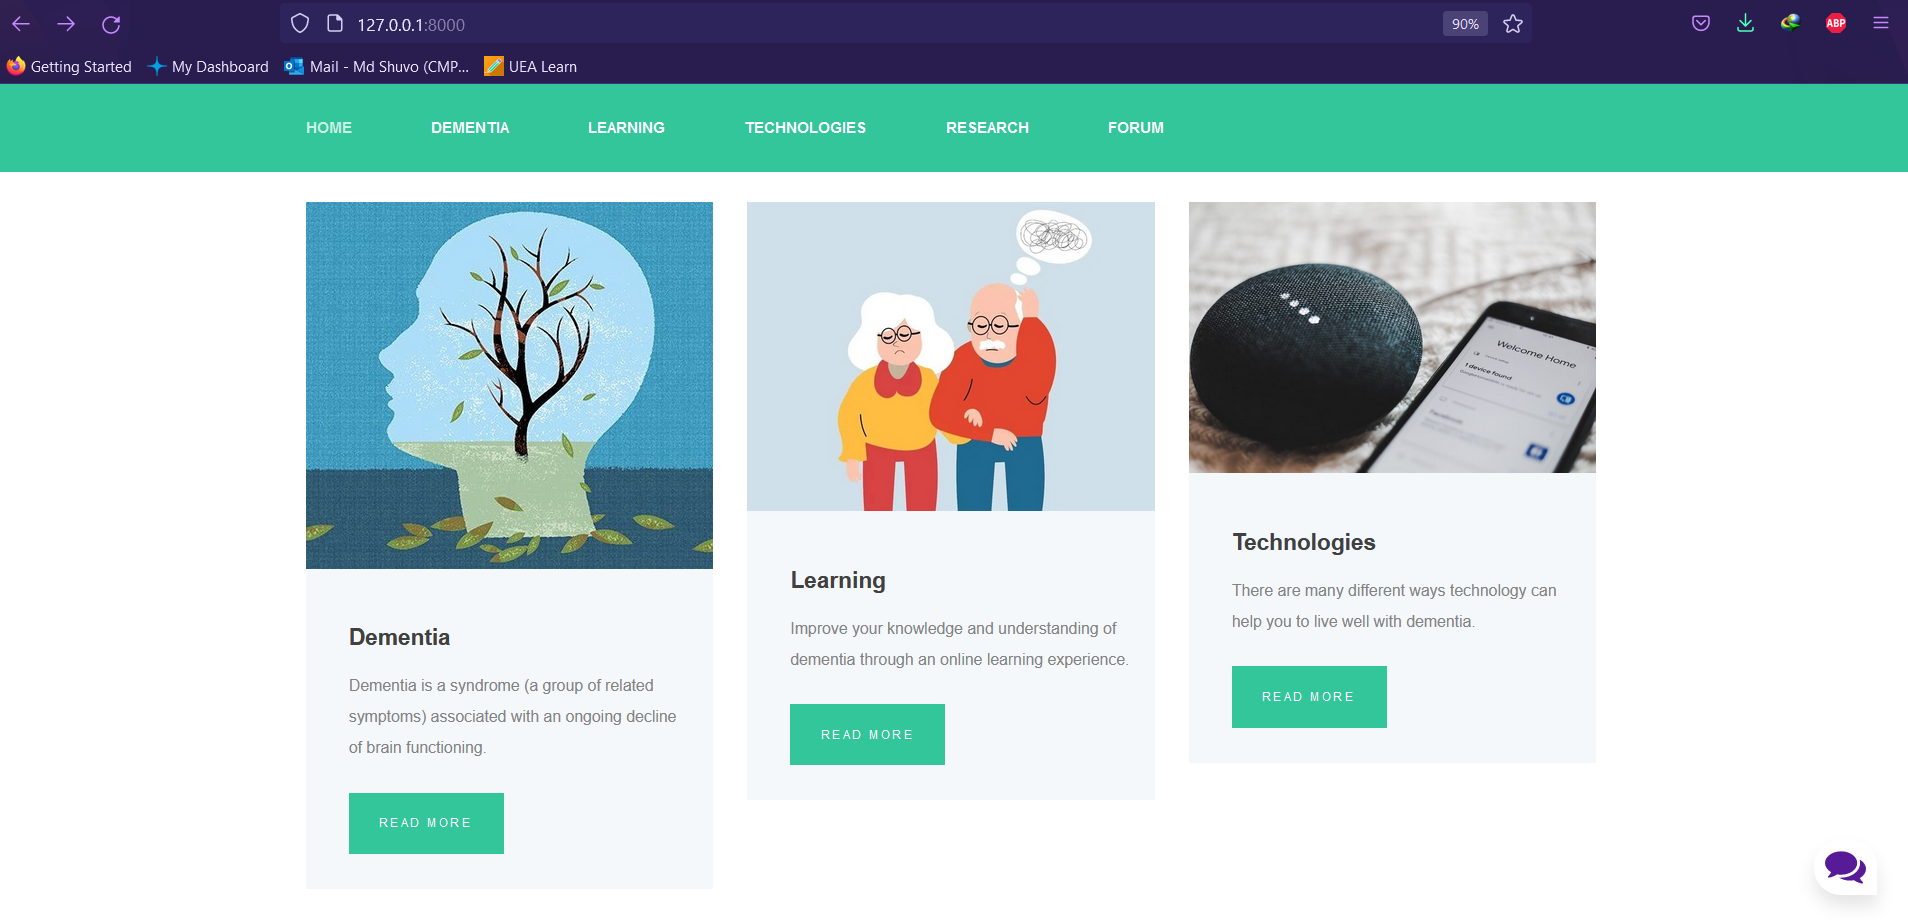
\includegraphics[width=0.85\textwidth]{home2}
	\caption{Homepage contains linked pages.}
	\label{fig:13}
\end{figure}

\begin{figure}[!h]
	\centering
	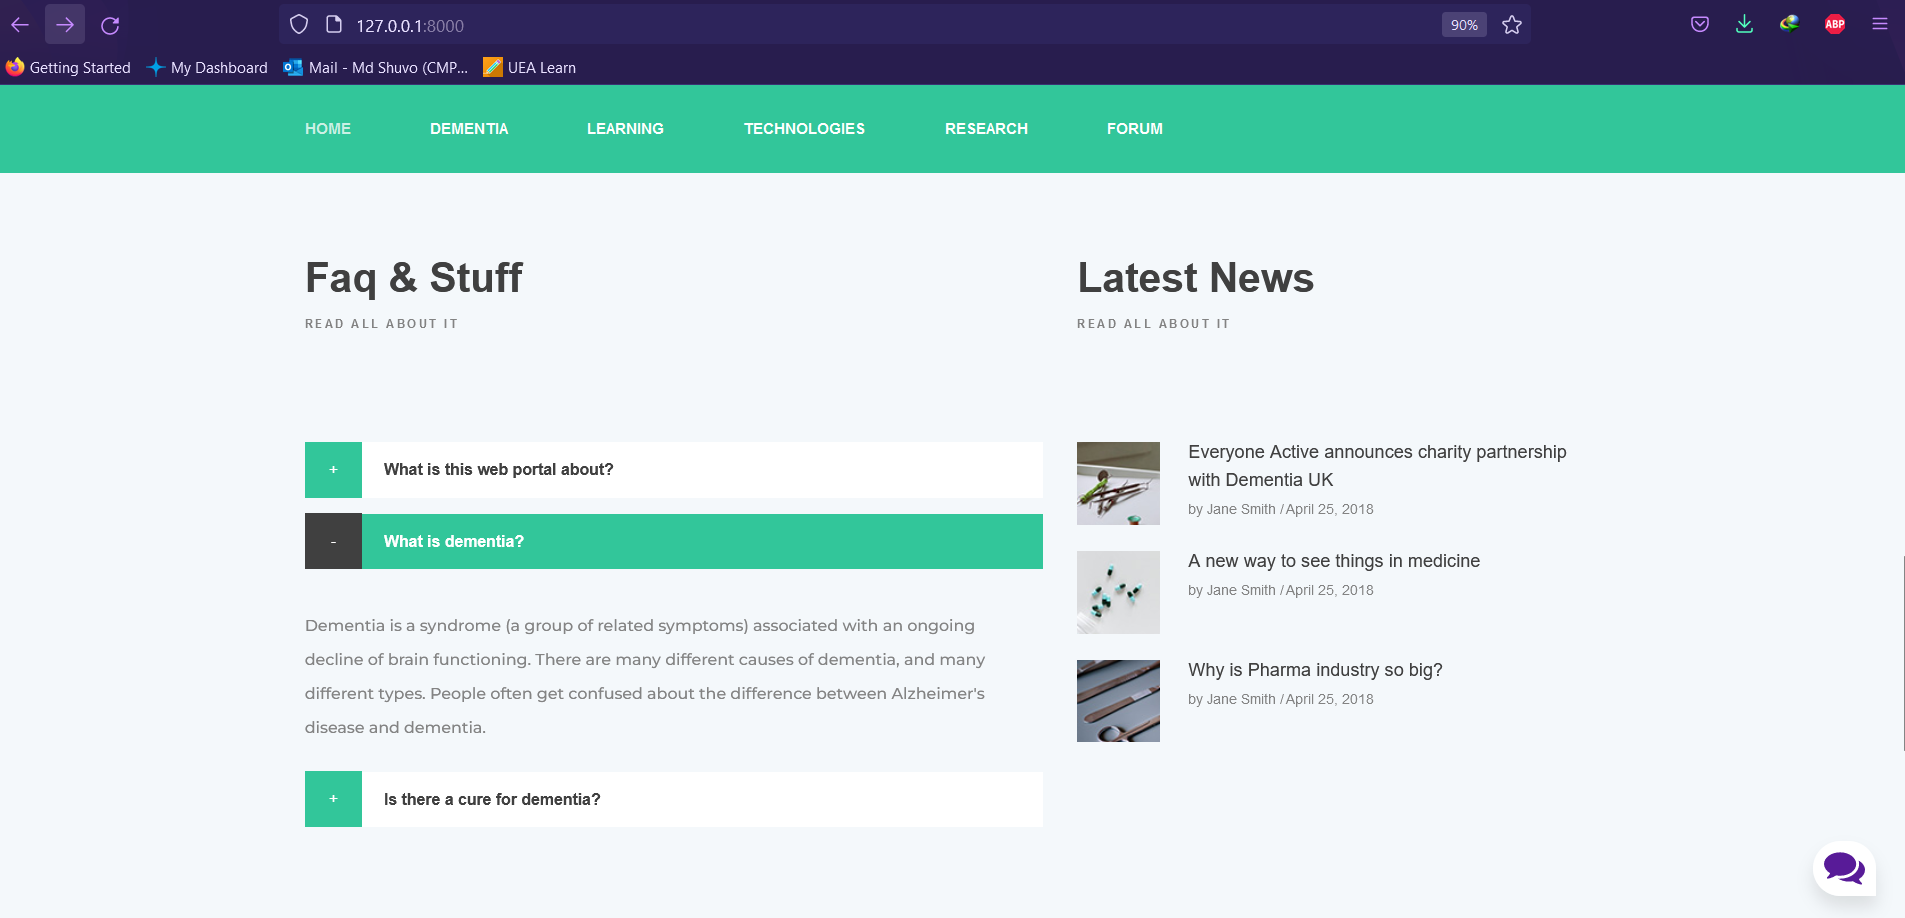
\includegraphics[width=0.85\textwidth]{home3}
	\caption{Homepage faq and recent articles.}
	\label{fig:14}
\end{figure}

\begin{figure}[!h]
	\centering
	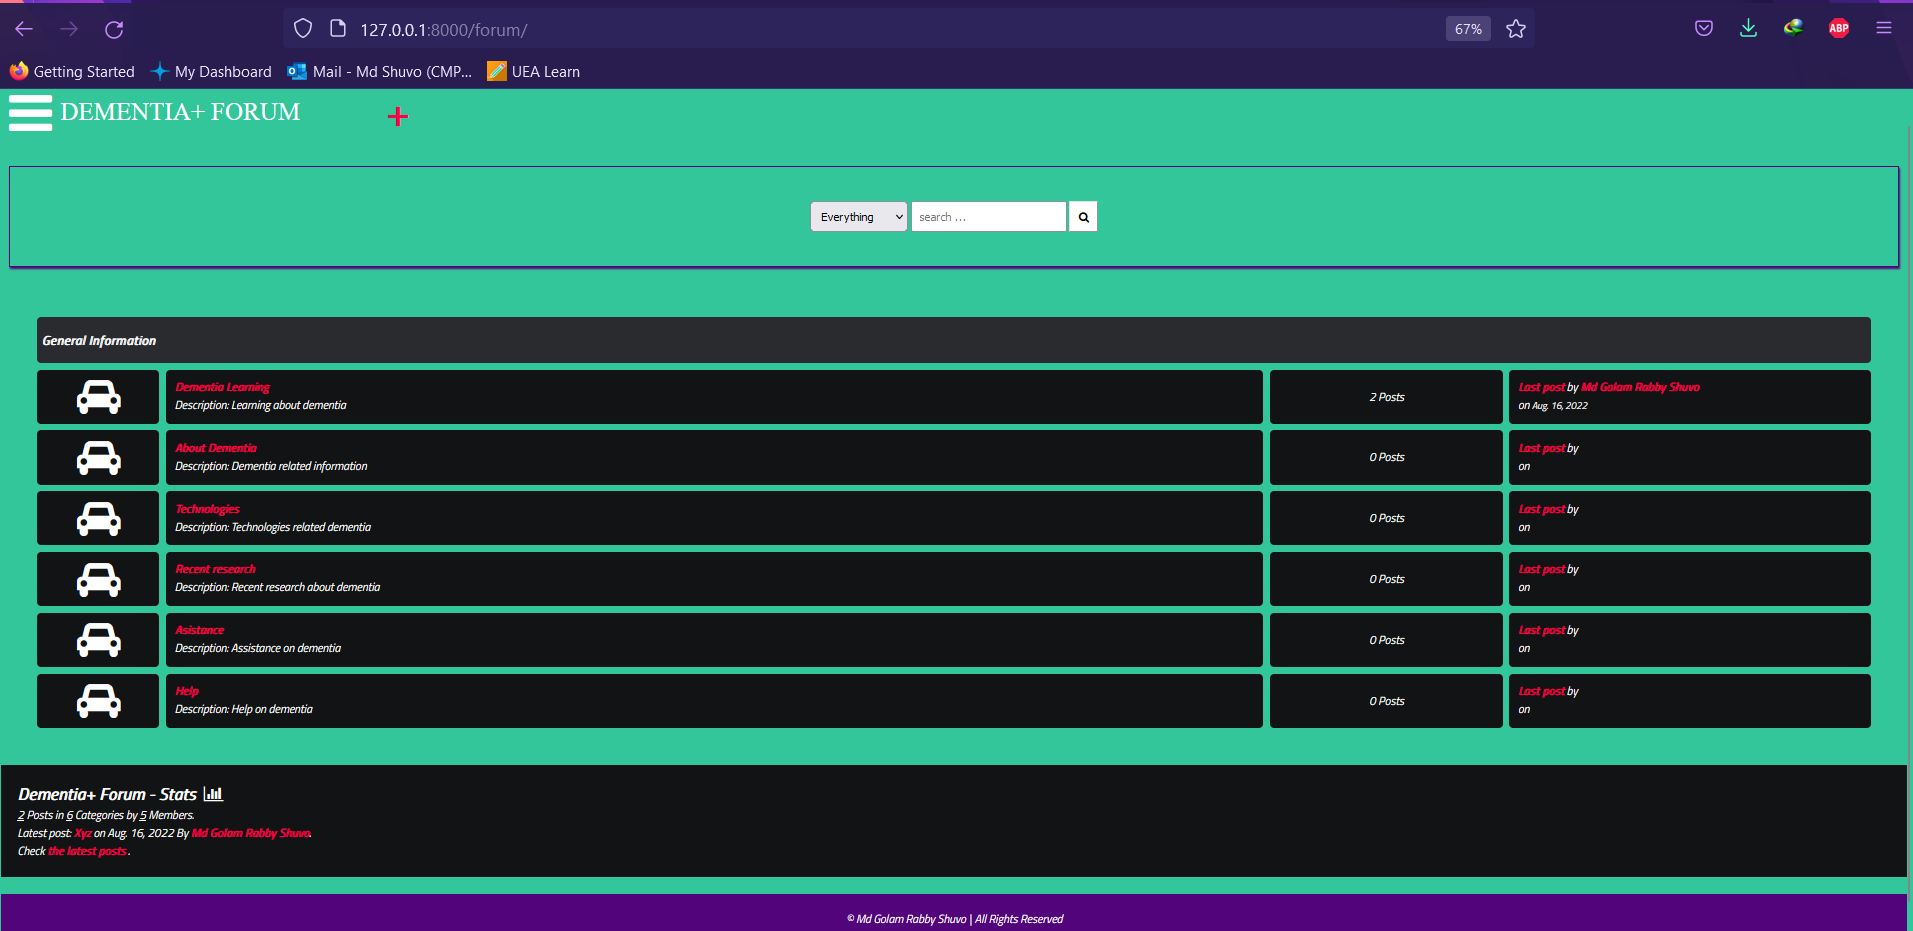
\includegraphics[width=0.85\textwidth]{forum}
	\caption{Forum homepage.}
	\label{fig:15}
\end{figure}

\begin{figure}[!h]
	\centering
	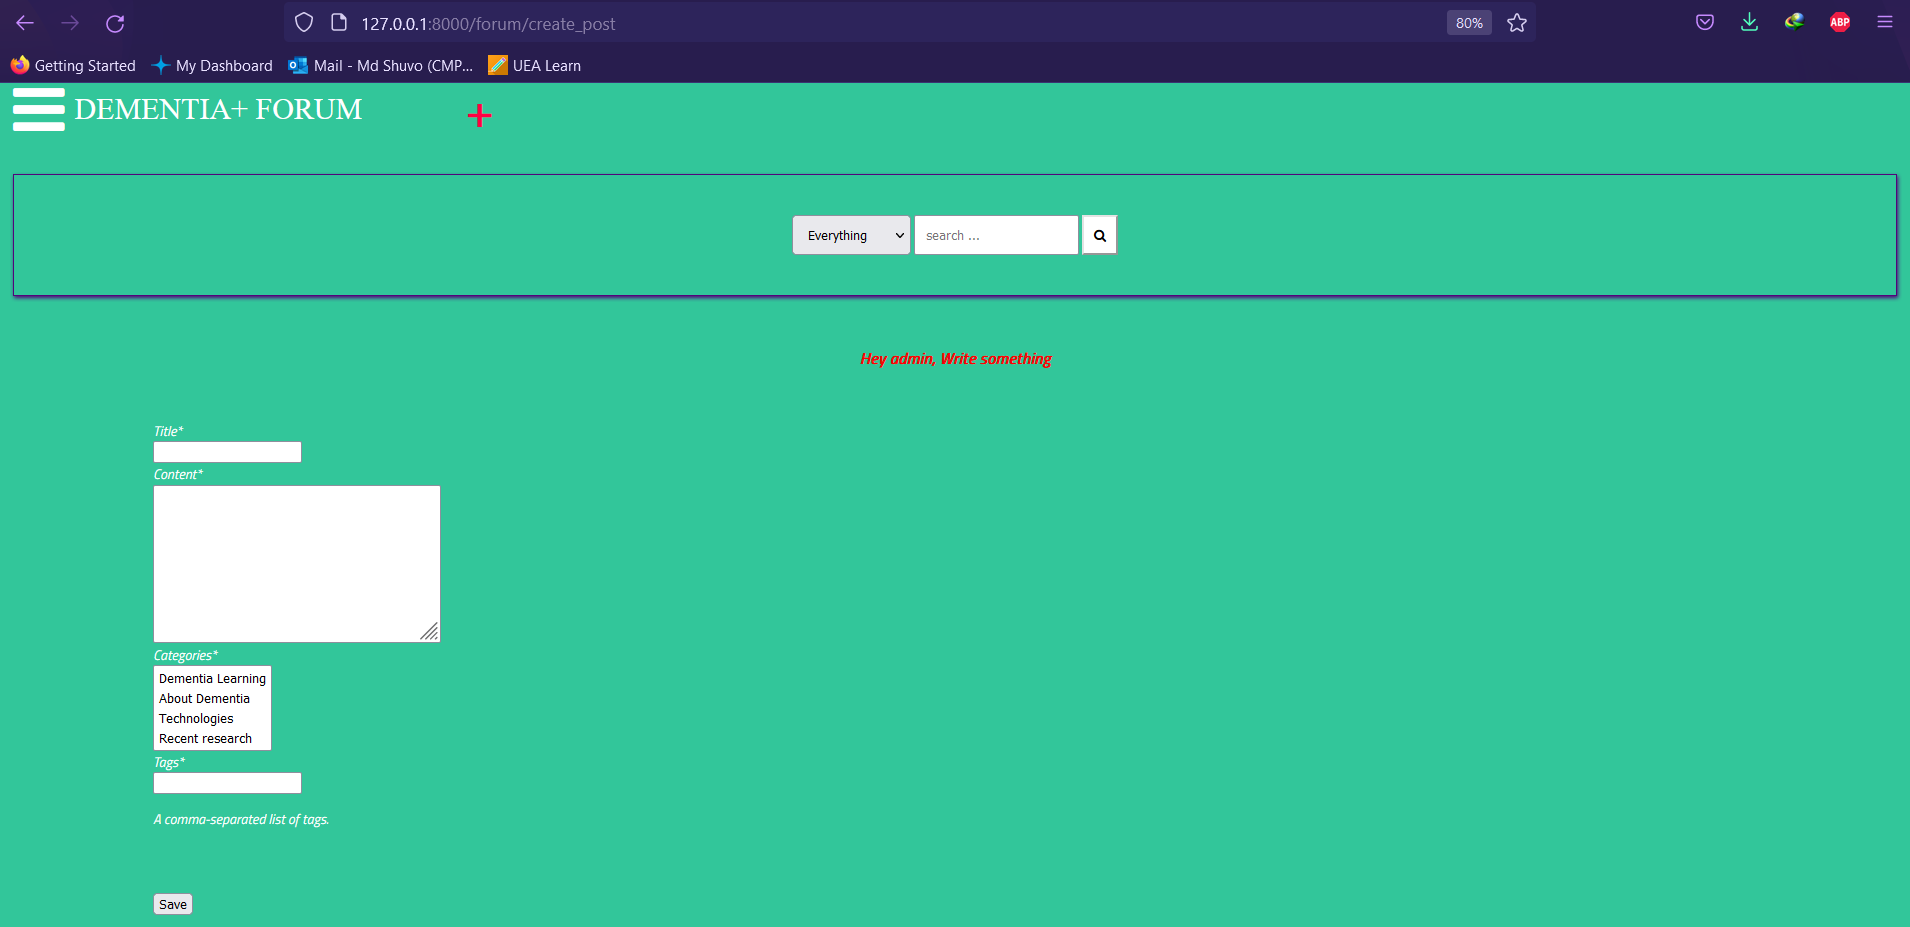
\includegraphics[width=0.85\textwidth]{create_post}
	\caption{Create post page.}
	\label{fig:16}
\end{figure}

\begin{figure}[!h]
	\centering
	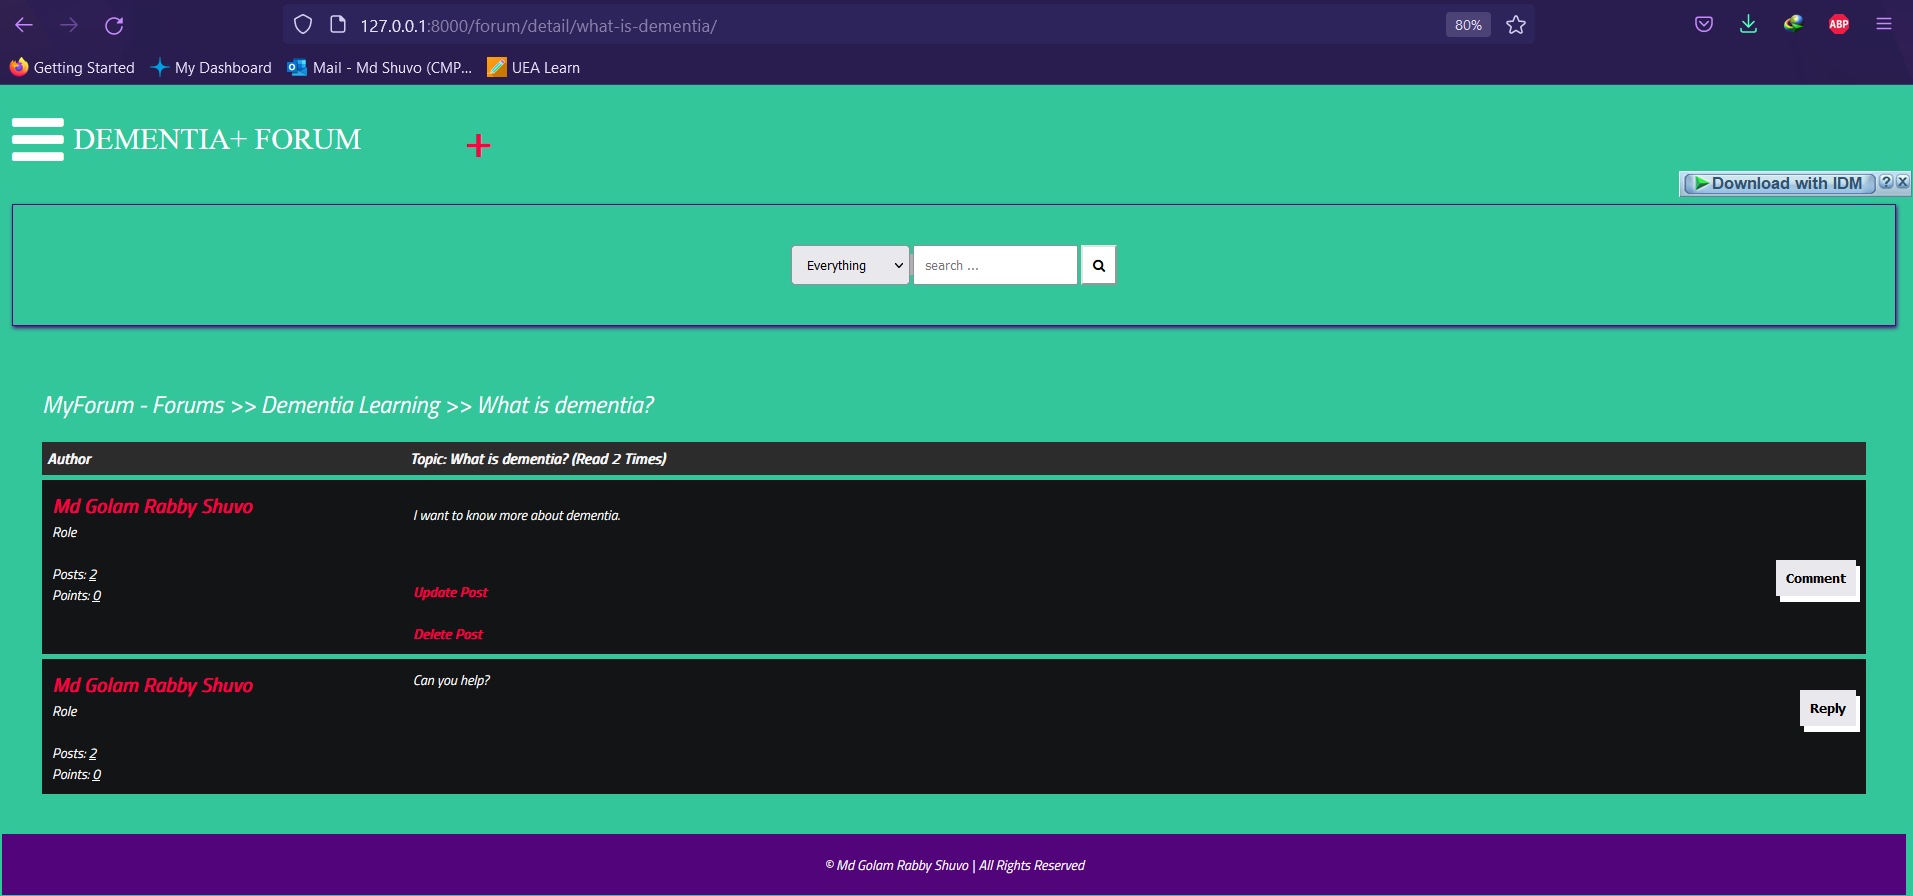
\includegraphics[width=0.85\textwidth]{post}
	\caption{A simple post.}
	\label{fig:17}
\end{figure}

\begin{figure}[!h]
	\centering
	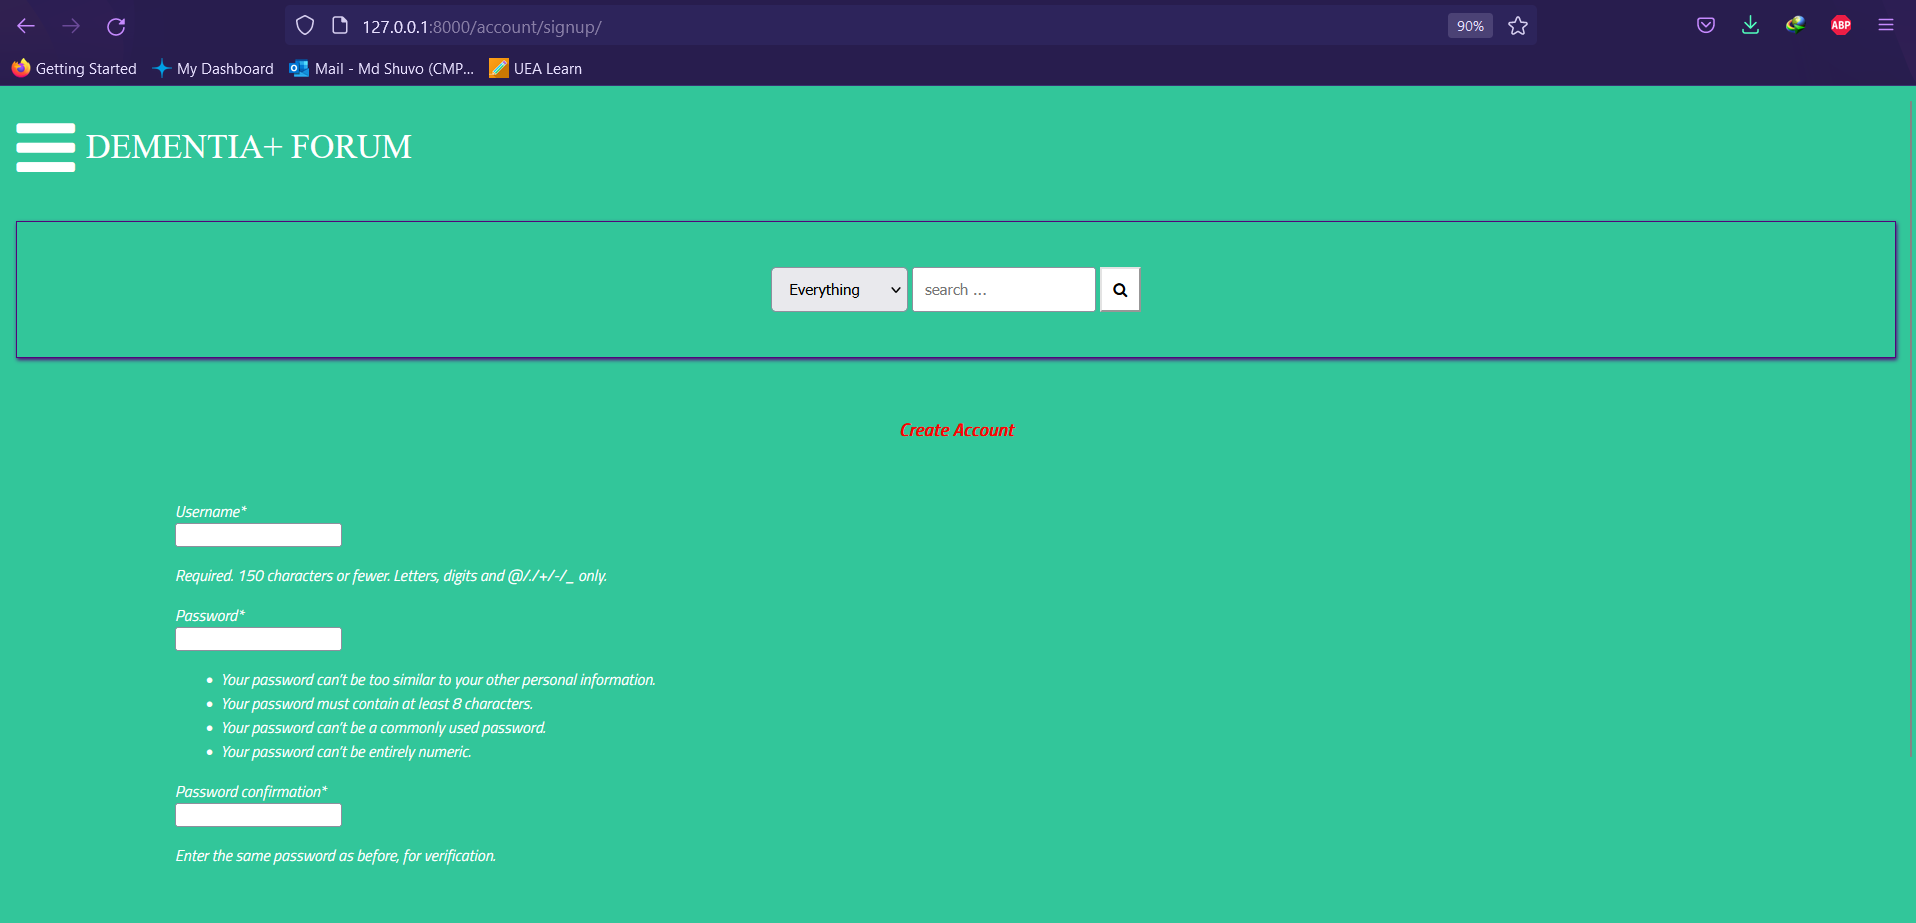
\includegraphics[width=0.85\textwidth]{signup}
	\caption{Signup page.}
	\label{fig:18}
\end{figure}

\begin{figure*}[ht!]
	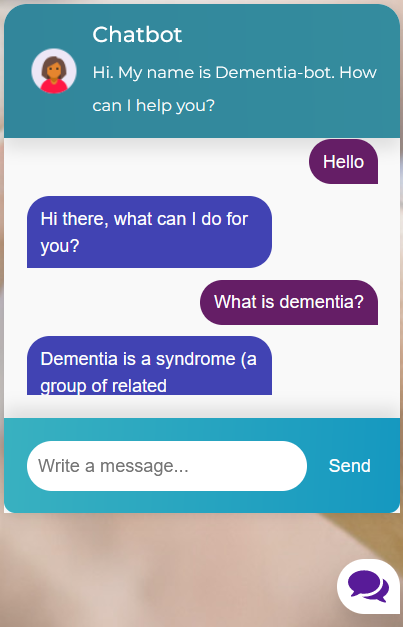
\includegraphics[width=.4\textwidth]{chat1}\hfill
	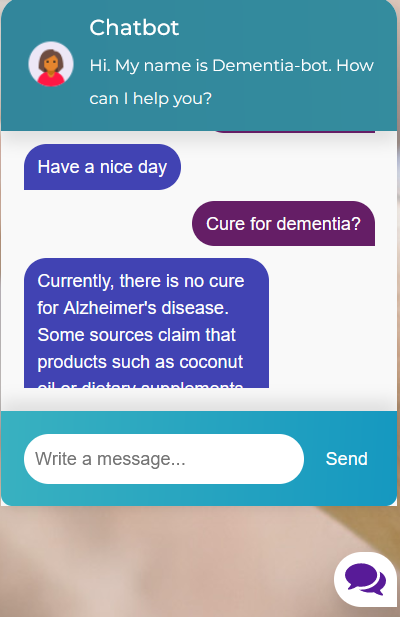
\includegraphics[width=.4\textwidth]{chat2}\hfill
	\caption{Chatbot in action.}
\end{figure*}

\def\baselinestretch{1.66}

%%% ----------------------------------------------------------------------
 

%%% ----------------------------------------------------------------------

 
%\include{Ch5}
%\include{Ch6} 
% ......
%\include{EvaluationAndDiscussion}
% ------------------------------------------------------------------------
% -*-TeX-*- -*-Hard-*- Smart Wrapping
% ------------------------------------------------------------------------
\def\baselinestretch{1}

\chapter{Conclusion}
This chapter explains evaluation, necessary discussion, conclusion summary and future work for my dissertation.

\def\baselinestretch{1.66}

%%% ----------------------------------------------------------------------
 

%%% ----------------------------------------------------------------------
\goodbreak
\section{Evaluation and Discussion}
An evaluation of software is a specific kind of assessment that is carried out with the purpose of determining whether or not a software programme or a collection of software applications is the sort of solution that is most suited to meeting the requirements of a certain customer. The purpose of this exercise is to take a closer look at the tools and resources that are made available by the application that is either being used at the moment by that client or is being considered as a potential addition to the programmes that are now being used by that client.

\subsection{Advantages of Chatbot}

\subsubsection{1. Available at any time:}
I'm sure the vast majority of you are routinely required to wait on hold as technicians link you to a customer care executive. They are taking the place of live chat as well as other, more time-consuming means of communication, such as emails and phone calls. Chatbots are essentially virtual robots, which means that they never grow tired and will continue to follow whatever instruction you give them. Your user experience (UX) will improve as a result, and you will climb the rankings in your industry. You also have the ability to expertly build your chatbot in order to keep your goal and emphasis in the right place, which is another benefit of this fast answer.

\subsubsection{2. Managing capability:}
Chat bots have the capacity to have discussions with thousands of individuals at the same time, in contrast to humans, who can only have a conversation with one other person at a time. Imagine that you are the owner of a restaurant that is well-known for the quality of its cuisine and that the majority of your profits come from delivery orders. You will have a greater number of clients to receive orders from, but you will only have a limited number of staff members to cater to all of these consumers. Having a chatbot will do rid of this issue, make it possible to attend to every single customer, and guarantee that no orders are overlooked. Chatbots are already being used by businesses such as Taco Bell and Domino's to coordinate the delivery of customers' packages.

\subsubsection{3. Characteristic of adaptability:}
The flexibility of chatbots makes them suitable for application in almost any sector because to their low entry barrier. Chatbots, in contrast to other products, for which switching platforms requires a significant amount of development work and testing, are quite simple to implement. It is sufficient to educate the bot by providing it with the appropriate discussion format and flow in order to alter the sector or industry in which it is currently operating.

\subsubsection{4. User appreciation:}
Emotional states fluctuate naturally in humans. Conversely, chatbots must follow the guidelines set forth for them in order to function properly. No matter how rude or profane a customer is, they will always be treated with the utmost professionalism. People's eating preferences might vary from day to day. In this situation, it may learn your address, offer recommendations for future purchases, and more based on your previous purchasing history.

\subsubsection{5. Economical and practical:}
It's never a cheap event to hire a person for a position, which will be considerably more costly if your revenues are not sufficient or sales objectives are not fulfilled, both of which would cause turmoil in the company. Because of the limitations that come with being human, a single person can only effectively interact with one or two other people at any given time. The employee would have a very difficult time if it were any higher than that. Chatbots could be able to assist in finding a solution to this age-old dilemma. Due to the fact that one chatbot is equivalent to a large number of workers, it is readily able to interact with thousands upon thousands of clients all at once. We would just need a small group of individuals to participate in chats here and there when it's really required.

\subsubsection{6. A quicker starting point:}
If you want to get anything done, you need to figure out how to do it first. They won't be qualified for the position unless they can demonstrate this. Every rung up the corporate ladder is accompanied by a new round of training for the individual in question. Not all workers will remain with the company, some will be let go, new ones will be hired, and so on. We seek to convey the reality that workers are subject to change. There will be a significant time investment on the part of existing staff in training the new hires. Chatbots have the potential to drastically reduce this wait time, but only if they follow a predetermined, human-friendly conversational format.

\subsection{Disadvantages of Chatbot}

\subsubsection{1. Inconveniently multi-purpose:}
Many programmers want to make a chatbot that can interact with any platform and function as a true personal assistant. However, practical bots end up not being able to handle the vast majority of questions. They have a number of drawbacks, including a tendency to misunderstand the users, forgetting what they were taught only 5 minutes before, etc. It's hardly surprising given that it takes a team of skilled programmers years to create a global bot that can interpret plain language and assess context. Additionally, even in this scenario, operational initiatives of this kind should be continuously enhanced.

\subsubsection{2. Simplistic Methods}
There are two distinct categories of bots: those that are powered by artificial intelligence and have the ability to pick up new skills via interaction, and those that are pre-programmed to respond appropriately in a variety of situations. Chatbots powered by artificial intelligence are said to be superior because of their ability to react differently based on the circumstances and the setting. However, the creation of intricate algorithms is necessary in order to accomplish this goal. In the meanwhile, only the largest companies in the information technology industry and a select few programmers have such a robust technical basis. As a result, it would be preferable for standard businesses to concentrate on the second kind of bots since they are more dependable and need less complexity. Due to the fact that they are lacking in intellect, it is quite unlikely that they will be able to engage in impolite modes of communication or break free from their creators' authority.

\subsubsection{3. Interface that is sophisticated:}
Conversation with a bot takes place in a chat environment, which requires the user to produce a significant amount of text. And in the event that the bot is unable to comprehend the user's request, it will be necessary for it to speak much more. It takes some time to determine which instructions a bot can answer to appropriately and which inquiries are best avoided in order to maximise its usefulness. Therefore, conversing with a chatbot will, in the vast majority of instances, not result in time savings. It's possible that in the not-too-distant future, virtual assistants may become even more useful thanks to the addition of a speech recognition capability. However, for the time being, its functional capabilities are quite limited, and there are only a select number of business domains in which they may be of any real value.

\subsection{Ethical, Social, and Legal Issues on Information Sharing}
Intelligent assistive technologies have a profound impact on patients’ emotional and psychosocial well-being because of their pervasiveness and ubiquitous nature. Dementia patients may benefit from personalized caring and assisted living technologies that allow them to remain within own homes and carry out daily tasks on their own \citep{leg1}. Correspondingly, owing to the technical uniqueness and complexity of intelligent tachnology for dementia, the incorporation of such systems into standard dementia care poses a series of legal and ethical difficulties. It has been suggested that the transition from humanistic to 13 technology-assisted care may have an unanticipated influence on the individual experience of elderly people living with dementia \citep{leg2}. Additional typical meta-ethical assessments for using intelligent technology in dementia care comprise the proper procurement of expressed permission \citep{leg3} and the safeguarding of individuals’ privacy rights from uninformed monitoring \citep{leg4}.

Although procurement and commissions play a critical role in the development of new ideas, legislative frameworks and inflexible organisational culture frequently lead to a risk-averse and limited approach to strategic purchase in the public sector. In addition, social care AI technology markets are still immature, making the integration of AI into social care delivery a challenging task. As a result of AI, social care may be provided at a lower cost and in a more personalised manner. Risk and reward are important considerations for contracting authority to make informed decisions. When it comes to AI technology and the data it generates, local governments must take additional steps to ensure that any commercial partnership is built on ethical foundations. When it comes to working with the commercial sector, local governments and care providers have a lot of knowledge that may be tapped upon as AI becomes more ubiquitous in social care. It is possible, however, for organisations to take further steps to guarantee that they connect with like-minded partners from the corporate sector, especially in terms of ethics and their commitment to social value.

\subsubsection{Risk factors}
The impact of AI on a broad variety of risk categories has grown in the last two years, including model and compliance risks as well as operational and legal risks as well as reputational and regulatory risks. Fresh and uncharted territory for those who have never used data analysis or model management in their businesses. Despite this, even in companies which possess a tradition of addressing these risks, AI presents these risks in unique and difficult ways. Investigators are still unable to verify the privacy and security of apps for Alzeimer's Disease (AD) or related conditions (AD/RD). Privacy breaches are more likely to occur because of the patient group's cognitive impairment and old age. Future studies will focus on privacy policies and the protection of user data. Because the MARS evaluation was not explicitly intended for AD/RD care–related applications, the researchers were able to capture some difference between both the apps and the MARS assessment. While other AD/RD care applications focus more on functionality, MARS places an emphasis on user involvement.

%\bigskip

%%% ----------------------------------------------------------------------
\goodbreak
\section{Conclusion}
Despite the significant progress that has been made, there is still a long way to go in the creation of intelligent technology that may be utilised in the treatment of dementia. This is the case despite the fact that there has been great progress. There has been a great deal of discourse over the role that assistive technology plays in the delivery of modern healthcare ever since the number of articles, conferences, and workshops that are specifically devoted to this topic has skyrocketed over the course of the last decade. In the years to come, it will be essential for academics and physicians to evaluate the performance attributes and usability of commercial items that originate from these projects in "real world" circumstances. Because of the growing interest among academics in this industry, there has been an increase in the number of national finance mechanisms that specifically investigate the applications of transdisciplinary technology research. However, there is no study of this kind on the construction of intelligent portals for dementia care. This research will aid a significant number of individuals in the healthcare industry, especially those working in dementia care.

%%% ----------------------------------------------------------------------
\goodbreak
\section{Suggestion for Further Work}
Any software, regardless of its current state, can almost always be made better. In the not-too-distant future, we could be expanded to incorporate more functions like File Transfer and Voice Message. It is feasible to make it as user-friendly as is humanly conceivable. It is important to us that it be created for the aim of producing money, and we would also want to give it a web domain. Due to the fact that the code is mostly organised or modular in nature, additional needs and upgrades may be simply implemented. Improvements may be appended by either modifying the modules that are already there or introducing new modules. It is possible to make more improvements to the application so that the website performs in a way that is more appealing to the user and helpful than the current one.

The potential of chatbots is still being explored, but their existing capabilities have their limits. Chatbots are not able to realise their full potential because of the constraints placed on the processing and retrieval of data. It's not for a lack of computer processing capacity on our end; we have enough of that. Nevertheless, there is a restriction on "How" we go about doing it. The market for customers who shop at retail establishments is one of the most prominent examples. Because of the nature of their requirements, clients at retail establishments are most interested in engaging with other people. They do not want their requirements to be analysed by bots and answered accordingly.

 

% ------------------------------------------------------------------------
\setlinespacing{1.44}
%\bibliographystyle{amsplain}
\bibliographystyle{apalike}
\bibliography{xbib} % use your own bib file

%#### Include any appendix below #####
\appendix

% MATH -------------------------------------------------------------------
\newcommand{\A}{{\cal A}}
\newcommand{\h}{{\cal H}}
\newcommand{\s}{{\cal S}}
\newcommand{\W}{{\cal W}}
\newcommand{\BH}{\mathbf B(\cal H)}
\newcommand{\KH}{\cal  K(\cal H)}
\newcommand{\Real}{\mathbb R}
\newcommand{\Complex}{\mathbb C}
\newcommand{\Field}{\mathbb F}
\newcommand{\RPlus}{[0,\infty)}
%
\newcommand{\norm}[1]{\left\Vert#1\right\Vert}
\newcommand{\essnorm}[1]{\norm{#1}_{\text{\rm\normalshape ess}}}
\newcommand{\abs}[1]{\left\vert#1\right\vert}
\newcommand{\set}[1]{\left\{#1\right\}}
\newcommand{\seq}[1]{\left<#1\right>}
\newcommand{\eps}{\varepsilon}
\newcommand{\To}{\longrightarrow}
\newcommand{\RE}{\operatorname{Re}}
\newcommand{\IM}{\operatorname{Im}}
\newcommand{\Poly}{{\cal{P}}(E)}
\newcommand{\EssD}{{\cal{D}}}
% THEOREMS ---------------------------------------------------------------
\theoremstyle{plain}
\newtheorem{thm}{Theorem}[section]
\newtheorem{cor}[thm]{Corollary}
\newtheorem{lem}[thm]{Lemma}
\newtheorem{prop}[thm]{Proposition}

\theoremstyle{definition}
\newtheorem{defn}{Definition}[section]
%
\theoremstyle{remark}
\newtheorem{rem}{Remark}[section]
%
\def\baselinestretch{1}

\chapter{List of dependencies requirements}

\def\baselinestretch{1.66}

%%% ----------------------------------------------------------------------
\begin{table}[!h]
	\centering
	\begin{tabular}{ |c|c| }
		\hline
		Number & Dependency \\
		\hline
		1 & asgiref==3.3.1 \\
		2 & astroid==2.4.2 \\
		3 & autopep8==1.5.4 \\
		4 & certifi==2020.12.5 \\
		5 & chardet==4.0.0 \\
		6 & colorama==0.4.4 \\
		7 & Django==3.1.4 \\
		8 & django-crispy-forms \\
		9 & django-filter==2.4.0 \\
		10 & djangorestframework==3.12.2 \\
		11 & django-hitcount \\
		12 & django-resized \\
		13 & django-taggit \\
		14 & django-tinymce \\
		15 & gunicorn==20.1.0 \\
		16 & idna==2.10 \\
		17 & isort==5.6.4 \\
		18 & lazy-object-proxy==1.4.3 \\
		19 & mccabe==0.6.1 \\
		20 & pycodestyle==2.6.0 \\
		21 & pylint==2.6.0 \\
		22 & python-dotenv==0.15.0 \\
		23 & pytz==2020.4 \\
		24 & requests==2.25.1 \\
		25 & six==1.15.0 \\
		26 & sqlparse==0.4.1 \\
		27 & toml==0.10.2 \\
		28 & urllib3==1.26.2 \\
		29 & whitenoise==6.2.0 \\
		30 & wrapt==1.12.1 \\
		\hline
	\end{tabular}
	\caption{Required dependencies for website.}
	\label{table:4}
\end{table}


%%% ----------------------------------------------------------------------
\goodbreak


\smallskip

\goodbreak

% ------------------------------------------------------------------------

%\include{AppendixB}

% =================================================================
\end{document}
% ------------------------------------------------------------------------
